\documentclass[twoside]{book}

% Packages required by doxygen
\usepackage{calc}
\usepackage{doxygen}
\usepackage{graphicx}
\usepackage[utf8]{inputenc}
\usepackage{makeidx}
\usepackage{multicol}
\usepackage{multirow}
\usepackage{textcomp}
\usepackage[table]{xcolor}

% Font selection
\usepackage[T1]{fontenc}
\usepackage{mathptmx}
\usepackage[scaled=.90]{helvet}
\usepackage{courier}
\usepackage{amssymb}
\usepackage{sectsty}
\renewcommand{\familydefault}{\sfdefault}
\allsectionsfont{%
  \fontseries{bc}\selectfont%
  \color{darkgray}%
}
\renewcommand{\DoxyLabelFont}{%
  \fontseries{bc}\selectfont%
  \color{darkgray}%
}

% Page & text layout
\usepackage{geometry}
\geometry{%
  a4paper,%
  top=2.5cm,%
  bottom=2.5cm,%
  left=2.5cm,%
  right=2.5cm%
}
\tolerance=750
\hfuzz=15pt
\hbadness=750
\setlength{\emergencystretch}{15pt}
\setlength{\parindent}{0cm}
\setlength{\parskip}{0.2cm}
\makeatletter
\renewcommand{\paragraph}{%
  \@startsection{paragraph}{4}{0ex}{-1.0ex}{1.0ex}{%
    \normalfont\normalsize\bfseries\SS@parafont%
  }%
}
\renewcommand{\subparagraph}{%
  \@startsection{subparagraph}{5}{0ex}{-1.0ex}{1.0ex}{%
    \normalfont\normalsize\bfseries\SS@subparafont%
  }%
}
\makeatother

% Headers & footers
\usepackage{fancyhdr}
\pagestyle{fancyplain}
\fancyhead[LE]{\fancyplain{}{\bfseries\thepage}}
\fancyhead[CE]{\fancyplain{}{}}
\fancyhead[RE]{\fancyplain{}{\bfseries\leftmark}}
\fancyhead[LO]{\fancyplain{}{\bfseries\rightmark}}
\fancyhead[CO]{\fancyplain{}{}}
\fancyhead[RO]{\fancyplain{}{\bfseries\thepage}}
\fancyfoot[LE]{\fancyplain{}{}}
\fancyfoot[CE]{\fancyplain{}{}}
\fancyfoot[RE]{\fancyplain{}{\bfseries\scriptsize Generated on Wed Apr 8 2015 18\-:25\-:06 for Lab03 -\/ podstawowe struktury danych\-: tablice(praca na programie kolegi) by Doxygen }}
\fancyfoot[LO]{\fancyplain{}{\bfseries\scriptsize Generated on Wed Apr 8 2015 18\-:25\-:06 for Lab03 -\/ podstawowe struktury danych\-: tablice(praca na programie kolegi) by Doxygen }}
\fancyfoot[CO]{\fancyplain{}{}}
\fancyfoot[RO]{\fancyplain{}{}}
\renewcommand{\footrulewidth}{0.4pt}
\renewcommand{\chaptermark}[1]{%
  \markboth{#1}{}%
}
\renewcommand{\sectionmark}[1]{%
  \markright{\thesection\ #1}%
}

% Indices & bibliography
\usepackage{natbib}
\usepackage[titles]{tocloft}
\setcounter{tocdepth}{3}
\setcounter{secnumdepth}{5}
\makeindex

% Hyperlinks (required, but should be loaded last)
\usepackage{ifpdf}
\ifpdf
  \usepackage[pdftex,pagebackref=true]{hyperref}
\else
  \usepackage[ps2pdf,pagebackref=true]{hyperref}
\fi
\hypersetup{%
  colorlinks=true,%
  linkcolor=blue,%
  citecolor=blue,%
  unicode%
}

% Custom commands
\newcommand{\clearemptydoublepage}{%
  \newpage{\pagestyle{empty}\cleardoublepage}%
}


%===== C O N T E N T S =====

\begin{document}

% Titlepage & ToC
\hypersetup{pageanchor=false}
\pagenumbering{roman}
\begin{titlepage}
\vspace*{7cm}
\begin{center}%
{\Large Lab03 -\/ podstawowe struktury danych\-: tablice(praca na programie kolegi) }\\
\vspace*{1cm}
{\large Generated by Doxygen 1.8.6}\\
\vspace*{0.5cm}
{\small Wed Apr 8 2015 18:25:06}\\
\end{center}
\end{titlepage}
\clearemptydoublepage
\tableofcontents
\clearemptydoublepage
\pagenumbering{arabic}
\hypersetup{pageanchor=true}

%--- Begin generated contents ---
\chapter{Namespace Index}
\section{Lista przestrzeni nazw}
Tutaj znajdują się wszystkie przestrzenie nazw wraz z ich krótkimi opisami\-:\begin{DoxyCompactList}
\item\contentsline{section}{\hyperlink{namespacearr}{arr} }{\pageref{namespacearr}}{}
\item\contentsline{section}{\hyperlink{namespacels}{ls} \\*\hyperlink{classls_1_1_kolejka}{Kolejka}, abstrakcyjna struktura danych z buforem typu L\-I\-F\-O }{\pageref{namespacels}}{}
\end{DoxyCompactList}

\chapter{Hierarchical Index}
\section{Class Hierarchy}
This inheritance list is sorted roughly, but not completely, alphabetically\-:\begin{DoxyCompactList}
\item \contentsline{section}{Dane}{\pageref{class_dane}}{}
\begin{DoxyCompactList}
\item \contentsline{section}{Pobieracz\-Danych}{\pageref{class_pobieracz_danych}}{}
\end{DoxyCompactList}
\item \contentsline{section}{Ekolejka}{\pageref{struct_ekolejka}}{}
\item \contentsline{section}{Element}{\pageref{struct_element}}{}
\item \contentsline{section}{Graf}{\pageref{class_graf}}{}
\item \contentsline{section}{Kolejka}{\pageref{class_kolejka}}{}
\item \contentsline{section}{Ltab}{\pageref{class_ltab}}{}
\item \contentsline{section}{Obserwowany}{\pageref{class_obserwowany}}{}
\begin{DoxyCompactList}
\item \contentsline{section}{Obserwator}{\pageref{class_obserwator}}{}
\end{DoxyCompactList}
\item \contentsline{section}{Stos}{\pageref{class_stos}}{}
\end{DoxyCompactList}

\chapter{Class Index}
\section{Class List}
Here are the classes, structs, unions and interfaces with brief descriptions\-:\begin{DoxyCompactList}
\item\contentsline{section}{{\bf cegla} \\*Struktura pomocnicza cegla }{\pageref{structcegla}}{}
\item\contentsline{section}{{\bf ls\-::\-Kolejka} }{\pageref{classls_1_1_kolejka}}{}
\item\contentsline{section}{{\bf arr\-::\-Kolejka} }{\pageref{classarr_1_1_kolejka}}{}
\item\contentsline{section}{{\bf ls\-::\-Kontener} }{\pageref{classls_1_1_kontener}}{}
\item\contentsline{section}{{\bf arr\-::\-Lista} }{\pageref{classarr_1_1_lista}}{}
\item\contentsline{section}{{\bf ls\-::\-Stos} }{\pageref{classls_1_1_stos}}{}
\item\contentsline{section}{{\bf arr\-::\-Stos} }{\pageref{classarr_1_1_stos}}{}
\end{DoxyCompactList}

\chapter{File Index}
\section{File List}
Here is a list of all files with brief descriptions\-:\begin{DoxyCompactList}
\item\contentsline{section}{/home/damian/prog/praca na zajeciach(nowy sort)/\-Sortowania(wybrany-\/przez wstawianie)/prj/inc/\hyperlink{_lista_ar_8h}{Lista\-Ar.\-h} \\*Plik naglowkowy \hyperlink{_lista_ar_8h}{Lista\-Ar.\-h} }{\pageref{_lista_ar_8h}}{}
\item\contentsline{section}{/home/damian/prog/praca na zajeciach(nowy sort)/\-Sortowania(wybrany-\/przez wstawianie)/prj/src/\hyperlink{_lista_ar_8cpp}{Lista\-Ar.\-cpp} \\*Plik \hyperlink{_lista_ar_8cpp}{Lista\-Ar.\-cpp} }{\pageref{_lista_ar_8cpp}}{}
\item\contentsline{section}{/home/damian/prog/praca na zajeciach(nowy sort)/\-Sortowania(wybrany-\/przez wstawianie)/prj/src/\hyperlink{main_8cpp}{main.\-cpp} \\*Plik \hyperlink{main_8cpp}{main.\-cpp} }{\pageref{main_8cpp}}{}
\end{DoxyCompactList}

\chapter{Namespace Documentation}
\hypertarget{namespacearr}{\section{arr Namespace Reference}
\label{namespacearr}\index{arr@{arr}}
}
\subsection*{Classes}
\begin{DoxyCompactItemize}
\item 
class \hyperlink{classarr_1_1_kolejka}{Kolejka}
\item 
class \hyperlink{classarr_1_1_lista}{Lista}
\item 
class \hyperlink{classarr_1_1_stos}{Stos}
\end{DoxyCompactItemize}

\hypertarget{namespacels}{\section{ls Namespace Reference}
\label{namespacels}\index{ls@{ls}}
}


\hyperlink{classls_1_1_kolejka}{Kolejka}, abstrakcyjna struktura danych z buforem typu L\-I\-F\-O.  


\subsection*{Classes}
\begin{DoxyCompactItemize}
\item 
class \hyperlink{classls_1_1_kolejka}{Kolejka}
\item 
class \hyperlink{classls_1_1_kontener}{Kontener}
\item 
class \hyperlink{classls_1_1_stos}{Stos}
\end{DoxyCompactItemize}


\subsection{Detailed Description}
\hyperlink{classls_1_1_stos}{Stos}, abstrakcyjna struktura danych z buforem typu F\-I\-F\-O. 
\chapter{Class Documentation}
\section{cegla Struct Reference}
\label{structcegla}\index{cegla@{cegla}}


Struktura pomocnicza cegla.  




{\ttfamily \#include $<$cegla.\-h$>$}

\subsection*{Public Member Functions}
\begin{DoxyCompactItemize}
\item 
{\bf cegla} ()
\end{DoxyCompactItemize}
\subsection*{Public Attributes}
\begin{DoxyCompactItemize}
\item 
int {\bf dana}
\item 
{\bf cegla} $\ast$ {\bf nastepna}
\end{DoxyCompactItemize}


\subsection{Detailed Description}
Struktura pomocnicza cegla. 

Struktura reprezentuje elementarną cząstkę kontenera -\/ zawiera daną oraz wskaźnik do kolejnego elementu w kontenerze. 

Definition at line 15 of file cegla.\-h.



\subsection{Constructor \& Destructor Documentation}
\index{cegla@{cegla}!cegla@{cegla}}
\index{cegla@{cegla}!cegla@{cegla}}
\subsubsection[{cegla}]{\setlength{\rightskip}{0pt plus 5cm}cegla\-::cegla (
\begin{DoxyParamCaption}
{}
\end{DoxyParamCaption}
)\hspace{0.3cm}{\ttfamily [inline]}}\label{structcegla_a7a8bf742844b4b9e526454cf49887e78}


Definition at line 19 of file cegla.\-h.



\subsection{Member Data Documentation}
\index{cegla@{cegla}!dana@{dana}}
\index{dana@{dana}!cegla@{cegla}}
\subsubsection[{dana}]{\setlength{\rightskip}{0pt plus 5cm}int cegla\-::dana}\label{structcegla_a25ba885f5ac99791f80fd1676ce22a3a}


Definition at line 17 of file cegla.\-h.

\index{cegla@{cegla}!nastepna@{nastepna}}
\index{nastepna@{nastepna}!cegla@{cegla}}
\subsubsection[{nastepna}]{\setlength{\rightskip}{0pt plus 5cm}{\bf cegla}$\ast$ cegla\-::nastepna}\label{structcegla_aca5144299572d01d919e2655e447f9a8}


Definition at line 18 of file cegla.\-h.



The documentation for this struct was generated from the following file\-:\begin{DoxyCompactItemize}
\item 
/home/damian/mkrawczuk/209147/lab03\-\_\-opt/prj/inc/{\bf cegla.\-h}\end{DoxyCompactItemize}

\hypertarget{classls_1_1_kolejka}{\section{Dokumentacja klasy ls\-:\-:Kolejka}
\label{classls_1_1_kolejka}\index{ls\-::\-Kolejka@{ls\-::\-Kolejka}}
}


{\ttfamily \#include $<$kolejka.\-h$>$}

Diagram dziedziczenia dla ls\-:\-:Kolejka\begin{figure}[H]
\begin{center}
\leavevmode
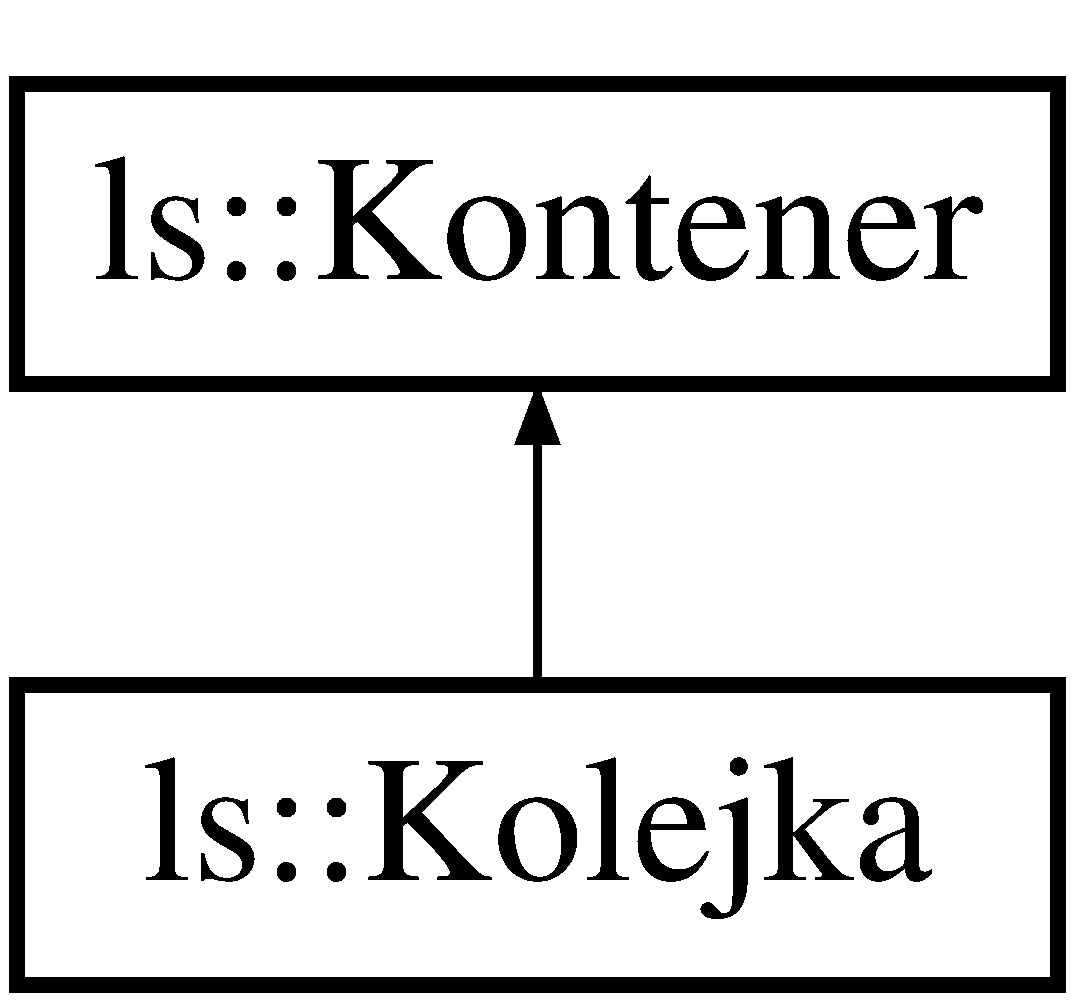
\includegraphics[height=2.000000cm]{classls_1_1_kolejka}
\end{center}
\end{figure}
\subsection*{Metody publiczne}
\begin{DoxyCompactItemize}
\item 
int \hyperlink{classls_1_1_kolejka_ac11693677f596b8a6dd2fc0183bbde90}{pop} ()
\begin{DoxyCompactList}\small\item\em Pop kolejki jaki jest, każdy widzi. Usuwa najstarszy element i zwraca wartość przez niego przechowywaną. \end{DoxyCompactList}\end{DoxyCompactItemize}
\subsection*{Dodatkowe Dziedziczone Składowe}


\subsection{Opis szczegółowy}


Definicja w linii 14 pliku kolejka.\-h.



\subsection{Dokumentacja funkcji składowych}
\hypertarget{classls_1_1_kolejka_ac11693677f596b8a6dd2fc0183bbde90}{\index{ls\-::\-Kolejka@{ls\-::\-Kolejka}!pop@{pop}}
\index{pop@{pop}!ls::Kolejka@{ls\-::\-Kolejka}}
\subsubsection[{pop}]{\setlength{\rightskip}{0pt plus 5cm}int ls\-::\-Kolejka\-::pop (
\begin{DoxyParamCaption}
{}
\end{DoxyParamCaption}
)\hspace{0.3cm}{\ttfamily [inline]}}}\label{classls_1_1_kolejka_ac11693677f596b8a6dd2fc0183bbde90}


Definicja w linii 21 pliku kolejka.\-h.



Dokumentacja dla tej klasy została wygenerowana z pliku\-:\begin{DoxyCompactItemize}
\item 
\hyperlink{kolejka_8h}{kolejka.\-h}\end{DoxyCompactItemize}

\hypertarget{classarr_1_1_kolejka}{\section{arr\-:\-:Kolejka Class Reference}
\label{classarr_1_1_kolejka}\index{arr\-::\-Kolejka@{arr\-::\-Kolejka}}
}


{\ttfamily \#include $<$kolejka\-\_\-arr.\-h$>$}

\subsection*{Public Member Functions}
\begin{DoxyCompactItemize}
\item 
\hyperlink{classarr_1_1_kolejka_a7f2d0e05c25b3a0d10db8e04cd4bdb58}{Kolejka} ()
\begin{DoxyCompactList}\small\item\em Konstruktor domyślny klasy \hyperlink{classarr_1_1_kolejka}{arr\-::\-Kolejka}. \end{DoxyCompactList}\item 
\hyperlink{classarr_1_1_kolejka_a1addd7f5fdee63f093fd971037600b02}{Kolejka} (const \hyperlink{classarr_1_1_kolejka}{Kolejka} \&lewy)
\begin{DoxyCompactList}\small\item\em Konstruktor kopiujący klasy \hyperlink{classarr_1_1_kolejka}{arr\-::\-Kolejka}. \end{DoxyCompactList}\item 
\hyperlink{classarr_1_1_kolejka_a455a5aac4ea9612cab749b8e9edf131d}{$\sim$\-Kolejka} ()
\begin{DoxyCompactList}\small\item\em Destruktor klasy \hyperlink{classarr_1_1_kolejka}{arr\-::\-Kolejka}. \end{DoxyCompactList}\item 
void \hyperlink{classarr_1_1_kolejka_acb08e887411da797ab39960cde892dc5}{push} (int val)
\begin{DoxyCompactList}\small\item\em Wrzuca element na szczyt kolejki. \end{DoxyCompactList}\item 
int \hyperlink{classarr_1_1_kolejka_a9d2c0676d6992ffb3b2aa4cd27ca36af}{pop} ()
\begin{DoxyCompactList}\small\item\em Zdejmuje najstarszy element z kolejki. \end{DoxyCompactList}\item 
bool \hyperlink{classarr_1_1_kolejka_a8ed4d617d36bf539544d1f7e18929bf8}{empty} ()
\begin{DoxyCompactList}\small\item\em Sprawdza, czy kolejka jest pusta. \end{DoxyCompactList}\item 
int \hyperlink{classarr_1_1_kolejka_a1aabde2dffcb50f4d8dc2e7d6df808ce}{size} ()
\begin{DoxyCompactList}\small\item\em Zwraca rozmiar kolejki. \end{DoxyCompactList}\end{DoxyCompactItemize}
\subsection*{Private Member Functions}
\begin{DoxyCompactItemize}
\item 
void \hyperlink{classarr_1_1_kolejka_affc094df5944c66cecfcaaeb490b7d67}{rozszerz\-\_\-x2} ()
\begin{DoxyCompactList}\small\item\em Metoda zwiększa dwukrotnie pojemnosć kolejki. \end{DoxyCompactList}\item 
void \hyperlink{classarr_1_1_kolejka_a05e15597ec59b3c77ba15112b4018b2f}{rozszerz\-\_\-1} ()
\begin{DoxyCompactList}\small\item\em Metoda zwiększa pojemnosć kolejki o 1. \end{DoxyCompactList}\end{DoxyCompactItemize}
\subsection*{Private Attributes}
\begin{DoxyCompactItemize}
\item 
int $\ast$ \hyperlink{classarr_1_1_kolejka_a80a504c56893e43ae1b407b971b501a7}{tablica}
\item 
int \hyperlink{classarr_1_1_kolejka_adbfdaca50c2b0bbe75d9b1e572f9b320}{rozmiar\-\_\-kol}
\item 
int \hyperlink{classarr_1_1_kolejka_ae10930beaa121ee5b178ffbb10b175e7}{pojemnosc\-\_\-kol}
\end{DoxyCompactItemize}


\subsection{Detailed Description}


Definition at line 7 of file kolejka\-\_\-arr.\-h.



\subsection{Constructor \& Destructor Documentation}
\hypertarget{classarr_1_1_kolejka_a7f2d0e05c25b3a0d10db8e04cd4bdb58}{\index{arr\-::\-Kolejka@{arr\-::\-Kolejka}!Kolejka@{Kolejka}}
\index{Kolejka@{Kolejka}!arr::Kolejka@{arr\-::\-Kolejka}}
\subsubsection[{Kolejka}]{\setlength{\rightskip}{0pt plus 5cm}arr\-::\-Kolejka\-::\-Kolejka (
\begin{DoxyParamCaption}
{}
\end{DoxyParamCaption}
)\hspace{0.3cm}{\ttfamily [inline]}}}\label{classarr_1_1_kolejka_a7f2d0e05c25b3a0d10db8e04cd4bdb58}


Definition at line 26 of file kolejka\-\_\-arr.\-h.

\hypertarget{classarr_1_1_kolejka_a1addd7f5fdee63f093fd971037600b02}{\index{arr\-::\-Kolejka@{arr\-::\-Kolejka}!Kolejka@{Kolejka}}
\index{Kolejka@{Kolejka}!arr::Kolejka@{arr\-::\-Kolejka}}
\subsubsection[{Kolejka}]{\setlength{\rightskip}{0pt plus 5cm}arr\-::\-Kolejka\-::\-Kolejka (
\begin{DoxyParamCaption}
\item[{const {\bf Kolejka} \&}]{lewy}
\end{DoxyParamCaption}
)}}\label{classarr_1_1_kolejka_a1addd7f5fdee63f093fd971037600b02}
Bezużyteczny dla trzeciego zadania, ale na pewno kolega się ucieszy. 

Definition at line 3 of file kolejka\-\_\-arr.\-cpp.

\hypertarget{classarr_1_1_kolejka_a455a5aac4ea9612cab749b8e9edf131d}{\index{arr\-::\-Kolejka@{arr\-::\-Kolejka}!$\sim$\-Kolejka@{$\sim$\-Kolejka}}
\index{$\sim$\-Kolejka@{$\sim$\-Kolejka}!arr::Kolejka@{arr\-::\-Kolejka}}
\subsubsection[{$\sim$\-Kolejka}]{\setlength{\rightskip}{0pt plus 5cm}arr\-::\-Kolejka\-::$\sim$\-Kolejka (
\begin{DoxyParamCaption}
{}
\end{DoxyParamCaption}
)}}\label{classarr_1_1_kolejka_a455a5aac4ea9612cab749b8e9edf131d}


Definition at line 10 of file kolejka\-\_\-arr.\-cpp.



\subsection{Member Function Documentation}
\hypertarget{classarr_1_1_kolejka_a8ed4d617d36bf539544d1f7e18929bf8}{\index{arr\-::\-Kolejka@{arr\-::\-Kolejka}!empty@{empty}}
\index{empty@{empty}!arr::Kolejka@{arr\-::\-Kolejka}}
\subsubsection[{empty}]{\setlength{\rightskip}{0pt plus 5cm}bool arr\-::\-Kolejka\-::empty (
\begin{DoxyParamCaption}
{}
\end{DoxyParamCaption}
)}}\label{classarr_1_1_kolejka_a8ed4d617d36bf539544d1f7e18929bf8}
\begin{DoxyReturn}{Returns}
Zwraca prawdę, jeżeli kolejka jest pusta. W przeciwnym razie zwraca false. 
\end{DoxyReturn}


Definition at line 44 of file kolejka\-\_\-arr.\-cpp.

\hypertarget{classarr_1_1_kolejka_a9d2c0676d6992ffb3b2aa4cd27ca36af}{\index{arr\-::\-Kolejka@{arr\-::\-Kolejka}!pop@{pop}}
\index{pop@{pop}!arr::Kolejka@{arr\-::\-Kolejka}}
\subsubsection[{pop}]{\setlength{\rightskip}{0pt plus 5cm}int arr\-::\-Kolejka\-::pop (
\begin{DoxyParamCaption}
{}
\end{DoxyParamCaption}
)}}\label{classarr_1_1_kolejka_a9d2c0676d6992ffb3b2aa4cd27ca36af}
\begin{DoxyReturn}{Returns}
Zwraca wartość przechowywaną w zdejmowanej cegiełce 
\end{DoxyReturn}


Definition at line 32 of file kolejka\-\_\-arr.\-cpp.

\hypertarget{classarr_1_1_kolejka_acb08e887411da797ab39960cde892dc5}{\index{arr\-::\-Kolejka@{arr\-::\-Kolejka}!push@{push}}
\index{push@{push}!arr::Kolejka@{arr\-::\-Kolejka}}
\subsubsection[{push}]{\setlength{\rightskip}{0pt plus 5cm}void arr\-::\-Kolejka\-::push (
\begin{DoxyParamCaption}
\item[{int}]{val}
\end{DoxyParamCaption}
)}}\label{classarr_1_1_kolejka_acb08e887411da797ab39960cde892dc5}


Definition at line 15 of file kolejka\-\_\-arr.\-cpp.

\hypertarget{classarr_1_1_kolejka_a05e15597ec59b3c77ba15112b4018b2f}{\index{arr\-::\-Kolejka@{arr\-::\-Kolejka}!rozszerz\-\_\-1@{rozszerz\-\_\-1}}
\index{rozszerz\-\_\-1@{rozszerz\-\_\-1}!arr::Kolejka@{arr\-::\-Kolejka}}
\subsubsection[{rozszerz\-\_\-1}]{\setlength{\rightskip}{0pt plus 5cm}void arr\-::\-Kolejka\-::rozszerz\-\_\-1 (
\begin{DoxyParamCaption}
{}
\end{DoxyParamCaption}
)\hspace{0.3cm}{\ttfamily [private]}}}\label{classarr_1_1_kolejka_a05e15597ec59b3c77ba15112b4018b2f}


Definition at line 64 of file kolejka\-\_\-arr.\-cpp.

\hypertarget{classarr_1_1_kolejka_affc094df5944c66cecfcaaeb490b7d67}{\index{arr\-::\-Kolejka@{arr\-::\-Kolejka}!rozszerz\-\_\-x2@{rozszerz\-\_\-x2}}
\index{rozszerz\-\_\-x2@{rozszerz\-\_\-x2}!arr::Kolejka@{arr\-::\-Kolejka}}
\subsubsection[{rozszerz\-\_\-x2}]{\setlength{\rightskip}{0pt plus 5cm}void arr\-::\-Kolejka\-::rozszerz\-\_\-x2 (
\begin{DoxyParamCaption}
{}
\end{DoxyParamCaption}
)\hspace{0.3cm}{\ttfamily [private]}}}\label{classarr_1_1_kolejka_affc094df5944c66cecfcaaeb490b7d67}


Definition at line 49 of file kolejka\-\_\-arr.\-cpp.

\hypertarget{classarr_1_1_kolejka_a1aabde2dffcb50f4d8dc2e7d6df808ce}{\index{arr\-::\-Kolejka@{arr\-::\-Kolejka}!size@{size}}
\index{size@{size}!arr::Kolejka@{arr\-::\-Kolejka}}
\subsubsection[{size}]{\setlength{\rightskip}{0pt plus 5cm}int arr\-::\-Kolejka\-::size (
\begin{DoxyParamCaption}
{}
\end{DoxyParamCaption}
)\hspace{0.3cm}{\ttfamily [inline]}}}\label{classarr_1_1_kolejka_a1aabde2dffcb50f4d8dc2e7d6df808ce}


Definition at line 56 of file kolejka\-\_\-arr.\-h.



\subsection{Member Data Documentation}
\hypertarget{classarr_1_1_kolejka_ae10930beaa121ee5b178ffbb10b175e7}{\index{arr\-::\-Kolejka@{arr\-::\-Kolejka}!pojemnosc\-\_\-kol@{pojemnosc\-\_\-kol}}
\index{pojemnosc\-\_\-kol@{pojemnosc\-\_\-kol}!arr::Kolejka@{arr\-::\-Kolejka}}
\subsubsection[{pojemnosc\-\_\-kol}]{\setlength{\rightskip}{0pt plus 5cm}int arr\-::\-Kolejka\-::pojemnosc\-\_\-kol\hspace{0.3cm}{\ttfamily [private]}}}\label{classarr_1_1_kolejka_ae10930beaa121ee5b178ffbb10b175e7}


Definition at line 12 of file kolejka\-\_\-arr.\-h.

\hypertarget{classarr_1_1_kolejka_adbfdaca50c2b0bbe75d9b1e572f9b320}{\index{arr\-::\-Kolejka@{arr\-::\-Kolejka}!rozmiar\-\_\-kol@{rozmiar\-\_\-kol}}
\index{rozmiar\-\_\-kol@{rozmiar\-\_\-kol}!arr::Kolejka@{arr\-::\-Kolejka}}
\subsubsection[{rozmiar\-\_\-kol}]{\setlength{\rightskip}{0pt plus 5cm}int arr\-::\-Kolejka\-::rozmiar\-\_\-kol\hspace{0.3cm}{\ttfamily [private]}}}\label{classarr_1_1_kolejka_adbfdaca50c2b0bbe75d9b1e572f9b320}


Definition at line 11 of file kolejka\-\_\-arr.\-h.

\hypertarget{classarr_1_1_kolejka_a80a504c56893e43ae1b407b971b501a7}{\index{arr\-::\-Kolejka@{arr\-::\-Kolejka}!tablica@{tablica}}
\index{tablica@{tablica}!arr::Kolejka@{arr\-::\-Kolejka}}
\subsubsection[{tablica}]{\setlength{\rightskip}{0pt plus 5cm}int$\ast$ arr\-::\-Kolejka\-::tablica\hspace{0.3cm}{\ttfamily [private]}}}\label{classarr_1_1_kolejka_a80a504c56893e43ae1b407b971b501a7}


Definition at line 10 of file kolejka\-\_\-arr.\-h.



The documentation for this class was generated from the following files\-:\begin{DoxyCompactItemize}
\item 
\hyperlink{kolejka__arr_8h}{kolejka\-\_\-arr.\-h}\item 
\hyperlink{kolejka__arr_8cpp}{kolejka\-\_\-arr.\-cpp}\end{DoxyCompactItemize}

\hypertarget{classls_1_1_kontener}{\section{Dokumentacja klasy ls\-:\-:Kontener}
\label{classls_1_1_kontener}\index{ls\-::\-Kontener@{ls\-::\-Kontener}}
}


{\ttfamily \#include $<$kontener.\-h$>$}

Diagram dziedziczenia dla ls\-:\-:Kontener\begin{figure}[H]
\begin{center}
\leavevmode
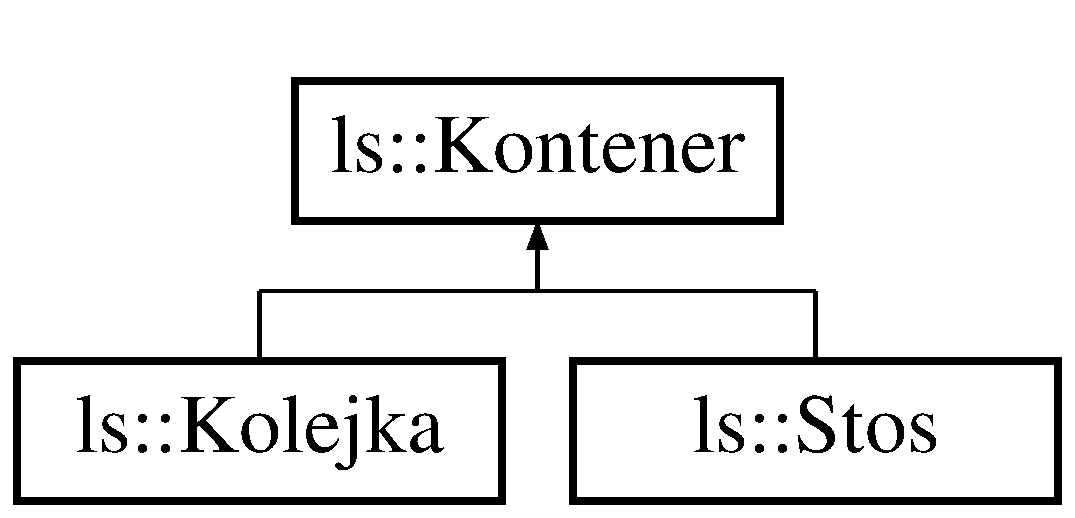
\includegraphics[height=2.000000cm]{classls_1_1_kontener}
\end{center}
\end{figure}
\subsection*{Metody publiczne}
\begin{DoxyCompactItemize}
\item 
\hyperlink{classls_1_1_kontener_a52711b1bc80413d48840ce8071a427fa}{$\sim$\-Kontener} ()
\begin{DoxyCompactList}\small\item\em Konstruktor klasy \hyperlink{classls_1_1_kontener}{Kontener}. \end{DoxyCompactList}\item 
\hyperlink{classls_1_1_kontener_a1c8f0e384b9d8e945ee70354eb144657}{Kontener} ()
\item 
void \hyperlink{classls_1_1_kontener_a911b275202510df1f321f8da26f0aa34}{push} (int)
\begin{DoxyCompactList}\small\item\em Wrzuca nową cegiełkę na początek kontenera. \end{DoxyCompactList}\item 
void \hyperlink{classls_1_1_kontener_a09517b6ec268d37744b1abbc7b7df5bb}{insert} (int wartosc, int indeks)
\begin{DoxyCompactList}\small\item\em Umieszcza cegłę z wartością 'wartosc' w miejscu oddalonym o 'indeks' miejsc od początku kontenera. \end{DoxyCompactList}\item 
int \hyperlink{classls_1_1_kontener_a248ac01db2477296b265fb0ea07a8c1c}{size} ()
\begin{DoxyCompactList}\small\item\em Liczy z ilu cegiełek składa się kontener. \end{DoxyCompactList}\item 
int \hyperlink{classls_1_1_kontener_a3b9fed0ce54e6232bd2868bf4b3801ec}{erase} (int)
\begin{DoxyCompactList}\small\item\em Usuwa z listy element o wybranym indeksie. \end{DoxyCompactList}\item 
int \hyperlink{classls_1_1_kontener_a04841df56a29d488e5e0d1a292646dde}{find} (int)
\begin{DoxyCompactList}\small\item\em Odnajduje w kontenerze przekazaną w argumencie wartość. \end{DoxyCompactList}\item 
void \hyperlink{classls_1_1_kontener_a75014b0a40e25ac573e2242d50522e08}{show} ()
\begin{DoxyCompactList}\small\item\em Wypisuje elementy listy od najmłodszego zaczynając. \end{DoxyCompactList}\end{DoxyCompactItemize}
\subsection*{Atrybuty chronione}
\begin{DoxyCompactItemize}
\item 
\hyperlink{structcegla}{cegla} $\ast$ \hyperlink{classls_1_1_kontener_af14ba3415f7ed315583ccb4575dfed9f}{alfa}
\end{DoxyCompactItemize}


\subsection{Opis szczegółowy}


Definicja w linii 14 pliku kontener.\-h.



\subsection{Dokumentacja konstruktora i destruktora}
\hypertarget{classls_1_1_kontener_a52711b1bc80413d48840ce8071a427fa}{\index{ls\-::\-Kontener@{ls\-::\-Kontener}!$\sim$\-Kontener@{$\sim$\-Kontener}}
\index{$\sim$\-Kontener@{$\sim$\-Kontener}!ls::Kontener@{ls\-::\-Kontener}}
\subsubsection[{$\sim$\-Kontener}]{\setlength{\rightskip}{0pt plus 5cm}ls\-::\-Kontener\-::$\sim$\-Kontener (
\begin{DoxyParamCaption}
{}
\end{DoxyParamCaption}
)}}\label{classls_1_1_kontener_a52711b1bc80413d48840ce8071a427fa}
Konstruktor klasy \hyperlink{classls_1_1_kontener}{Kontener} inicjalizuje wskaźnik 'alfa' wartością N\-U\-L\-L. 

Definicja w linii 7 pliku kontener.\-cpp.

\hypertarget{classls_1_1_kontener_a1c8f0e384b9d8e945ee70354eb144657}{\index{ls\-::\-Kontener@{ls\-::\-Kontener}!Kontener@{Kontener}}
\index{Kontener@{Kontener}!ls::Kontener@{ls\-::\-Kontener}}
\subsubsection[{Kontener}]{\setlength{\rightskip}{0pt plus 5cm}ls\-::\-Kontener\-::\-Kontener (
\begin{DoxyParamCaption}
{}
\end{DoxyParamCaption}
)\hspace{0.3cm}{\ttfamily [inline]}}}\label{classls_1_1_kontener_a1c8f0e384b9d8e945ee70354eb144657}


Definicja w linii 27 pliku kontener.\-h.



\subsection{Dokumentacja funkcji składowych}
\hypertarget{classls_1_1_kontener_a3b9fed0ce54e6232bd2868bf4b3801ec}{\index{ls\-::\-Kontener@{ls\-::\-Kontener}!erase@{erase}}
\index{erase@{erase}!ls::Kontener@{ls\-::\-Kontener}}
\subsubsection[{erase}]{\setlength{\rightskip}{0pt plus 5cm}int ls\-::\-Kontener\-::erase (
\begin{DoxyParamCaption}
\item[{int}]{indeks}
\end{DoxyParamCaption}
)}}\label{classls_1_1_kontener_a3b9fed0ce54e6232bd2868bf4b3801ec}
Zainicjalizowane są dwa wskaźniki na najmłodszą cegiełkę. Jeden jest ustawiany na element do usunięcia, drugi na element o jeden młodszy. Następuje roszada wskaźników\-: wskaźnik młodszej cegły wskazuje na cegłę starszą od usuwanej, zostaje zapisana wartość przechowywana przez usuwaną cegłę i wreszcie zwolniona zostaje pamięć zajmowana dotychczas przez cegłę.

Przykład 1\-: Wyrażenie obj.\-erase(0) usuwa najmłodszy element kontenera. Przykład 2\-: Wyrażenie obj.\-erase(obj.\-size() -\/ 1) usuwa najstarszy element. Przykład 3\-: Wyrażenie obj.\-erase(obj.\-size()) nie zmienia kontenera.

\begin{DoxyReturn}{Zwraca}
Zwraca wartość przechowywaną w usuniętej cegiełce. 
\end{DoxyReturn}


Definicja w linii 65 pliku kontener.\-cpp.

\hypertarget{classls_1_1_kontener_a04841df56a29d488e5e0d1a292646dde}{\index{ls\-::\-Kontener@{ls\-::\-Kontener}!find@{find}}
\index{find@{find}!ls::Kontener@{ls\-::\-Kontener}}
\subsubsection[{find}]{\setlength{\rightskip}{0pt plus 5cm}int ls\-::\-Kontener\-::find (
\begin{DoxyParamCaption}
\item[{int}]{wartosc}
\end{DoxyParamCaption}
)}}\label{classls_1_1_kontener_a04841df56a29d488e5e0d1a292646dde}
Powołany do życia jest szpieg -\/ wskaźnik na obiekt typu 'cegla', który przemierza kontener w poszukiwaniu najwcześniejszego wystąpienia poszukiwanej wartości. Operacji towarzyszy licznik, który śledzi ilość miniętych przez wskaźnik cegieł, którą metoda zwraca. Należy ją interpretować jako indeks cegły, gdzie najwcześniej wystąpiła poszukiwana wartość.

\begin{DoxyReturn}{Zwraca}
Zwraca indeks (liczony od 0 od najmłodszej cegiełki) najbliższego wystąpienia poszukiwanej wartości. 
\end{DoxyReturn}


Definicja w linii 99 pliku kontener.\-cpp.

\hypertarget{classls_1_1_kontener_a09517b6ec268d37744b1abbc7b7df5bb}{\index{ls\-::\-Kontener@{ls\-::\-Kontener}!insert@{insert}}
\index{insert@{insert}!ls::Kontener@{ls\-::\-Kontener}}
\subsubsection[{insert}]{\setlength{\rightskip}{0pt plus 5cm}void ls\-::\-Kontener\-::insert (
\begin{DoxyParamCaption}
\item[{int}]{wartosc, }
\item[{int}]{indeks}
\end{DoxyParamCaption}
)}}\label{classls_1_1_kontener_a09517b6ec268d37744b1abbc7b7df5bb}
U\-W\-A\-G\-A\-: Indeks liczony jest od zera, od najmłodszej cegły.

Przykład 1\-: Wyrażenie obj.\-insert(5,0) jest równoważne wyrażeniu obj.\-push(5)
\begin{DoxyItemize}
\item element zawierający wartość 5 jest teraz najmłodszym elementem. Przykład 2\-: Wyrażenie obj.\-insert(3,obj.\-size()) czyni element zawierający wartosć 3 najstarszym elementem. 
\end{DoxyItemize}

Definicja w linii 21 pliku kontener.\-cpp.

\hypertarget{classls_1_1_kontener_a911b275202510df1f321f8da26f0aa34}{\index{ls\-::\-Kontener@{ls\-::\-Kontener}!push@{push}}
\index{push@{push}!ls::Kontener@{ls\-::\-Kontener}}
\subsubsection[{push}]{\setlength{\rightskip}{0pt plus 5cm}void ls\-::\-Kontener\-::push (
\begin{DoxyParamCaption}
\item[{int}]{wart}
\end{DoxyParamCaption}
)}}\label{classls_1_1_kontener_a911b275202510df1f321f8da26f0aa34}


Definicja w linii 13 pliku kontener.\-cpp.

\hypertarget{classls_1_1_kontener_a75014b0a40e25ac573e2242d50522e08}{\index{ls\-::\-Kontener@{ls\-::\-Kontener}!show@{show}}
\index{show@{show}!ls::Kontener@{ls\-::\-Kontener}}
\subsubsection[{show}]{\setlength{\rightskip}{0pt plus 5cm}void ls\-::\-Kontener\-::show (
\begin{DoxyParamCaption}
{}
\end{DoxyParamCaption}
)}}\label{classls_1_1_kontener_a75014b0a40e25ac573e2242d50522e08}


Definicja w linii 116 pliku kontener.\-cpp.

\hypertarget{classls_1_1_kontener_a248ac01db2477296b265fb0ea07a8c1c}{\index{ls\-::\-Kontener@{ls\-::\-Kontener}!size@{size}}
\index{size@{size}!ls::Kontener@{ls\-::\-Kontener}}
\subsubsection[{size}]{\setlength{\rightskip}{0pt plus 5cm}int ls\-::\-Kontener\-::size (
\begin{DoxyParamCaption}
{}
\end{DoxyParamCaption}
)}}\label{classls_1_1_kontener_a248ac01db2477296b265fb0ea07a8c1c}
Zainicjalizowany zostaje wskaźnik na strukturę 'cegla' wskazujący na najmłodszą cegiełkę. Zostaje on potem wysłany w epicką podróż na sam koniec kontenera (czyli do napotkania N\-U\-L\-La). Towarzyszy mu licznik, który zlicza mijane po drodze cegiełki, których ilosć funkcja zwraca.

\begin{DoxyReturn}{Zwraca}
Zwraca wielkość kontenera. 
\end{DoxyReturn}


Definicja w linii 50 pliku kontener.\-cpp.



\subsection{Dokumentacja atrybutów składowych}
\hypertarget{classls_1_1_kontener_af14ba3415f7ed315583ccb4575dfed9f}{\index{ls\-::\-Kontener@{ls\-::\-Kontener}!alfa@{alfa}}
\index{alfa@{alfa}!ls::Kontener@{ls\-::\-Kontener}}
\subsubsection[{alfa}]{\setlength{\rightskip}{0pt plus 5cm}{\bf cegla}$\ast$ ls\-::\-Kontener\-::alfa\hspace{0.3cm}{\ttfamily [protected]}}}\label{classls_1_1_kontener_af14ba3415f7ed315583ccb4575dfed9f}


Definicja w linii 17 pliku kontener.\-h.



Dokumentacja dla tej klasy została wygenerowana z plików\-:\begin{DoxyCompactItemize}
\item 
\hyperlink{kontener_8h}{kontener.\-h}\item 
\hyperlink{kontener_8cpp}{kontener.\-cpp}\end{DoxyCompactItemize}

\hypertarget{classarr_1_1_lista}{\section{Dokumentacja klasy arr\-:\-:Lista}
\label{classarr_1_1_lista}\index{arr\-::\-Lista@{arr\-::\-Lista}}
}


{\ttfamily \#include $<$lista\-\_\-arr.\-h$>$}

\subsection*{Metody publiczne}
\begin{DoxyCompactItemize}
\item 
\hyperlink{classarr_1_1_lista_a11b61b647380e962aeeb35848c427b81}{Lista} ()
\begin{DoxyCompactList}\small\item\em Konstruktor domyślny klasy \hyperlink{classarr_1_1_lista}{arr\-::\-Lista}. \end{DoxyCompactList}\item 
\hyperlink{classarr_1_1_lista_a29bae0190a2d5c38ebfdf33eb05d1c09}{Lista} (const \hyperlink{classarr_1_1_lista}{Lista} \&lewy)
\begin{DoxyCompactList}\small\item\em Konstruktor kopiujący klasy \hyperlink{classarr_1_1_lista}{arr\-::\-Lista}. \end{DoxyCompactList}\item 
\hyperlink{classarr_1_1_lista_ac3b5f77b08befbf28e922179dcace594}{$\sim$\-Lista} ()
\begin{DoxyCompactList}\small\item\em Destruktor klasy \hyperlink{classarr_1_1_lista}{arr\-::\-Lista}. \end{DoxyCompactList}\item 
int \hyperlink{classarr_1_1_lista_ad370aa7f4e6bf3f2492f5187c9d64d56}{erase} (int)
\begin{DoxyCompactList}\small\item\em Usuwa z listy element o wybranym indeksie. \end{DoxyCompactList}\item 
void \hyperlink{classarr_1_1_lista_a57365c410ba6ac9d82eb4b4a83bc89bd}{insert} (int, int)
\begin{DoxyCompactList}\small\item\em Umieszcza cegłę z wartością 'wartosc' w miejscu oddalonym o 'indeks' miejsc od początku kontenera. \end{DoxyCompactList}\item 
bool \hyperlink{classarr_1_1_lista_a6eef5db974ccbb5f133a76d22b375ae9}{empty} ()
\begin{DoxyCompactList}\small\item\em Sprawdza, czy lista jest pusta. \end{DoxyCompactList}\item 
int \hyperlink{classarr_1_1_lista_a853418a2061e80c83185f03f0e1568c6}{size} ()
\begin{DoxyCompactList}\small\item\em Zwraca rozmiar listy. \end{DoxyCompactList}\end{DoxyCompactItemize}
\subsection*{Metody prywatne}
\begin{DoxyCompactItemize}
\item 
void \hyperlink{classarr_1_1_lista_ac4f01715efe075f780e006d757ed0c26}{rozszerz\-\_\-x2} ()
\begin{DoxyCompactList}\small\item\em Metoda zwiększa dwukrotnie pojemnosć listy. \end{DoxyCompactList}\item 
void \hyperlink{classarr_1_1_lista_ad6bf8061555507002920efbe6f3c0bb1}{rozszerz\-\_\-1} ()
\begin{DoxyCompactList}\small\item\em Metoda zwiększa pojemnosć listy o 1. \end{DoxyCompactList}\end{DoxyCompactItemize}
\subsection*{Atrybuty prywatne}
\begin{DoxyCompactItemize}
\item 
int $\ast$ \hyperlink{classarr_1_1_lista_aba76002ee48a3dc21187f0bf9da1a746}{tablica}
\item 
int \hyperlink{classarr_1_1_lista_a5d6712accdb4a0eda72038aadbfe1cd6}{rozmiar\-\_\-ls}
\item 
int \hyperlink{classarr_1_1_lista_a46550171712501ae7301b95b5c35d14c}{pojemnosc\-\_\-ls}
\end{DoxyCompactItemize}


\subsection{Opis szczegółowy}


Definicja w linii 6 pliku lista\-\_\-arr.\-h.



\subsection{Dokumentacja konstruktora i destruktora}
\hypertarget{classarr_1_1_lista_a11b61b647380e962aeeb35848c427b81}{\index{arr\-::\-Lista@{arr\-::\-Lista}!Lista@{Lista}}
\index{Lista@{Lista}!arr::Lista@{arr\-::\-Lista}}
\subsubsection[{Lista}]{\setlength{\rightskip}{0pt plus 5cm}arr\-::\-Lista\-::\-Lista (
\begin{DoxyParamCaption}
{}
\end{DoxyParamCaption}
)\hspace{0.3cm}{\ttfamily [inline]}}}\label{classarr_1_1_lista_a11b61b647380e962aeeb35848c427b81}


Definicja w linii 25 pliku lista\-\_\-arr.\-h.

\hypertarget{classarr_1_1_lista_a29bae0190a2d5c38ebfdf33eb05d1c09}{\index{arr\-::\-Lista@{arr\-::\-Lista}!Lista@{Lista}}
\index{Lista@{Lista}!arr::Lista@{arr\-::\-Lista}}
\subsubsection[{Lista}]{\setlength{\rightskip}{0pt plus 5cm}arr\-::\-Lista\-::\-Lista (
\begin{DoxyParamCaption}
\item[{const {\bf Lista} \&}]{lewy}
\end{DoxyParamCaption}
)}}\label{classarr_1_1_lista_a29bae0190a2d5c38ebfdf33eb05d1c09}
Bezużyteczny dla trzeciego zadania, ale na pewno kolega się ucieszy. \hypertarget{classarr_1_1_lista_ac3b5f77b08befbf28e922179dcace594}{\index{arr\-::\-Lista@{arr\-::\-Lista}!$\sim$\-Lista@{$\sim$\-Lista}}
\index{$\sim$\-Lista@{$\sim$\-Lista}!arr::Lista@{arr\-::\-Lista}}
\subsubsection[{$\sim$\-Lista}]{\setlength{\rightskip}{0pt plus 5cm}arr\-::\-Lista\-::$\sim$\-Lista (
\begin{DoxyParamCaption}
{}
\end{DoxyParamCaption}
)\hspace{0.3cm}{\ttfamily [inline]}}}\label{classarr_1_1_lista_ac3b5f77b08befbf28e922179dcace594}


Definicja w linii 35 pliku lista\-\_\-arr.\-h.



\subsection{Dokumentacja funkcji składowych}
\hypertarget{classarr_1_1_lista_a6eef5db974ccbb5f133a76d22b375ae9}{\index{arr\-::\-Lista@{arr\-::\-Lista}!empty@{empty}}
\index{empty@{empty}!arr::Lista@{arr\-::\-Lista}}
\subsubsection[{empty}]{\setlength{\rightskip}{0pt plus 5cm}bool arr\-::\-Lista\-::empty (
\begin{DoxyParamCaption}
{}
\end{DoxyParamCaption}
)}}\label{classarr_1_1_lista_a6eef5db974ccbb5f133a76d22b375ae9}
\begin{DoxyReturn}{Zwraca}
Zwraca prawdę, jeżeli lista jest pusta. W przeciwnym razie zwraca false. 
\end{DoxyReturn}


Definicja w linii 3 pliku lista\-\_\-arr.\-cpp.

\hypertarget{classarr_1_1_lista_ad370aa7f4e6bf3f2492f5187c9d64d56}{\index{arr\-::\-Lista@{arr\-::\-Lista}!erase@{erase}}
\index{erase@{erase}!arr::Lista@{arr\-::\-Lista}}
\subsubsection[{erase}]{\setlength{\rightskip}{0pt plus 5cm}int arr\-::\-Lista\-::erase (
\begin{DoxyParamCaption}
\item[{int}]{indeks}
\end{DoxyParamCaption}
)}}\label{classarr_1_1_lista_ad370aa7f4e6bf3f2492f5187c9d64d56}
Zapisuje wartość przechowywaną pod danym indeksem a potem przesuwa całą zawartość tablicy młodszą od danego elementu o 1 w stronę starszych elementów. Zmniejsza licznik rozmiar\-\_\-ls o 1.

Przykład 1\-: Wyrażenie obj.\-erase(0) usuwa najmłodszy element kontenera. Przykład 2\-: Wyrażenie obj.\-erase(obj.\-size() -\/ 1) usuwa najstarszy element. Przykład 3\-: Wyrażenie obj.\-erase(obj.\-size()) nie zmienia kontenera.

\begin{DoxyReturn}{Zwraca}
Zwraca wartość przechowywaną w usuniętej cegiełce. 
\end{DoxyReturn}


Definicja w linii 8 pliku lista\-\_\-arr.\-cpp.

\hypertarget{classarr_1_1_lista_a57365c410ba6ac9d82eb4b4a83bc89bd}{\index{arr\-::\-Lista@{arr\-::\-Lista}!insert@{insert}}
\index{insert@{insert}!arr::Lista@{arr\-::\-Lista}}
\subsubsection[{insert}]{\setlength{\rightskip}{0pt plus 5cm}void arr\-::\-Lista\-::insert (
\begin{DoxyParamCaption}
\item[{int}]{value, }
\item[{int}]{indeks}
\end{DoxyParamCaption}
)}}\label{classarr_1_1_lista_a57365c410ba6ac9d82eb4b4a83bc89bd}
Zwiększa licznik rozmiar\-\_\-ls o 1, odsuwa wszystkie elementy młodsze od danego indeksu o 1 od starszych i umieszcza wartość w odpowiednim indeksie. Może powodować realokację zawartości listy!

U\-W\-A\-G\-A\-: Indeks liczony jest od zera, od najmłodszej cegły.

Przykład 1\-: Wyrażenie obj.\-insert(5,0) jest równoważne wyrażeniu obj.\-push(5)
\begin{DoxyItemize}
\item element zawierający wartość 5 jest teraz najmłodszym elementem. Przykład 2\-: Wyrażenie obj.\-insert(3,obj.\-size()) czyni element zawierający wartosć 3 najstarszym elementem. 
\end{DoxyItemize}

Definicja w linii 20 pliku lista\-\_\-arr.\-cpp.

\hypertarget{classarr_1_1_lista_ad6bf8061555507002920efbe6f3c0bb1}{\index{arr\-::\-Lista@{arr\-::\-Lista}!rozszerz\-\_\-1@{rozszerz\-\_\-1}}
\index{rozszerz\-\_\-1@{rozszerz\-\_\-1}!arr::Lista@{arr\-::\-Lista}}
\subsubsection[{rozszerz\-\_\-1}]{\setlength{\rightskip}{0pt plus 5cm}void arr\-::\-Lista\-::rozszerz\-\_\-1 (
\begin{DoxyParamCaption}
{}
\end{DoxyParamCaption}
)\hspace{0.3cm}{\ttfamily [private]}}}\label{classarr_1_1_lista_ad6bf8061555507002920efbe6f3c0bb1}


Definicja w linii 59 pliku lista\-\_\-arr.\-cpp.

\hypertarget{classarr_1_1_lista_ac4f01715efe075f780e006d757ed0c26}{\index{arr\-::\-Lista@{arr\-::\-Lista}!rozszerz\-\_\-x2@{rozszerz\-\_\-x2}}
\index{rozszerz\-\_\-x2@{rozszerz\-\_\-x2}!arr::Lista@{arr\-::\-Lista}}
\subsubsection[{rozszerz\-\_\-x2}]{\setlength{\rightskip}{0pt plus 5cm}void arr\-::\-Lista\-::rozszerz\-\_\-x2 (
\begin{DoxyParamCaption}
{}
\end{DoxyParamCaption}
)\hspace{0.3cm}{\ttfamily [private]}}}\label{classarr_1_1_lista_ac4f01715efe075f780e006d757ed0c26}


Definicja w linii 44 pliku lista\-\_\-arr.\-cpp.

\hypertarget{classarr_1_1_lista_a853418a2061e80c83185f03f0e1568c6}{\index{arr\-::\-Lista@{arr\-::\-Lista}!size@{size}}
\index{size@{size}!arr::Lista@{arr\-::\-Lista}}
\subsubsection[{size}]{\setlength{\rightskip}{0pt plus 5cm}int arr\-::\-Lista\-::size (
\begin{DoxyParamCaption}
{}
\end{DoxyParamCaption}
)\hspace{0.3cm}{\ttfamily [inline]}}}\label{classarr_1_1_lista_a853418a2061e80c83185f03f0e1568c6}


Definicja w linii 83 pliku lista\-\_\-arr.\-h.



\subsection{Dokumentacja atrybutów składowych}
\hypertarget{classarr_1_1_lista_a46550171712501ae7301b95b5c35d14c}{\index{arr\-::\-Lista@{arr\-::\-Lista}!pojemnosc\-\_\-ls@{pojemnosc\-\_\-ls}}
\index{pojemnosc\-\_\-ls@{pojemnosc\-\_\-ls}!arr::Lista@{arr\-::\-Lista}}
\subsubsection[{pojemnosc\-\_\-ls}]{\setlength{\rightskip}{0pt plus 5cm}int arr\-::\-Lista\-::pojemnosc\-\_\-ls\hspace{0.3cm}{\ttfamily [private]}}}\label{classarr_1_1_lista_a46550171712501ae7301b95b5c35d14c}


Definicja w linii 11 pliku lista\-\_\-arr.\-h.

\hypertarget{classarr_1_1_lista_a5d6712accdb4a0eda72038aadbfe1cd6}{\index{arr\-::\-Lista@{arr\-::\-Lista}!rozmiar\-\_\-ls@{rozmiar\-\_\-ls}}
\index{rozmiar\-\_\-ls@{rozmiar\-\_\-ls}!arr::Lista@{arr\-::\-Lista}}
\subsubsection[{rozmiar\-\_\-ls}]{\setlength{\rightskip}{0pt plus 5cm}int arr\-::\-Lista\-::rozmiar\-\_\-ls\hspace{0.3cm}{\ttfamily [private]}}}\label{classarr_1_1_lista_a5d6712accdb4a0eda72038aadbfe1cd6}


Definicja w linii 10 pliku lista\-\_\-arr.\-h.

\hypertarget{classarr_1_1_lista_aba76002ee48a3dc21187f0bf9da1a746}{\index{arr\-::\-Lista@{arr\-::\-Lista}!tablica@{tablica}}
\index{tablica@{tablica}!arr::Lista@{arr\-::\-Lista}}
\subsubsection[{tablica}]{\setlength{\rightskip}{0pt plus 5cm}int$\ast$ arr\-::\-Lista\-::tablica\hspace{0.3cm}{\ttfamily [private]}}}\label{classarr_1_1_lista_aba76002ee48a3dc21187f0bf9da1a746}


Definicja w linii 9 pliku lista\-\_\-arr.\-h.



Dokumentacja dla tej klasy została wygenerowana z plików\-:\begin{DoxyCompactItemize}
\item 
\hyperlink{lista__arr_8h}{lista\-\_\-arr.\-h}\item 
\hyperlink{lista__arr_8cpp}{lista\-\_\-arr.\-cpp}\end{DoxyCompactItemize}

\hypertarget{classls_1_1_stos}{\section{ls\-:\-:Stos Class Reference}
\label{classls_1_1_stos}\index{ls\-::\-Stos@{ls\-::\-Stos}}
}


{\ttfamily \#include $<$stos.\-h$>$}

Inheritance diagram for ls\-:\-:Stos\-:\begin{figure}[H]
\begin{center}
\leavevmode
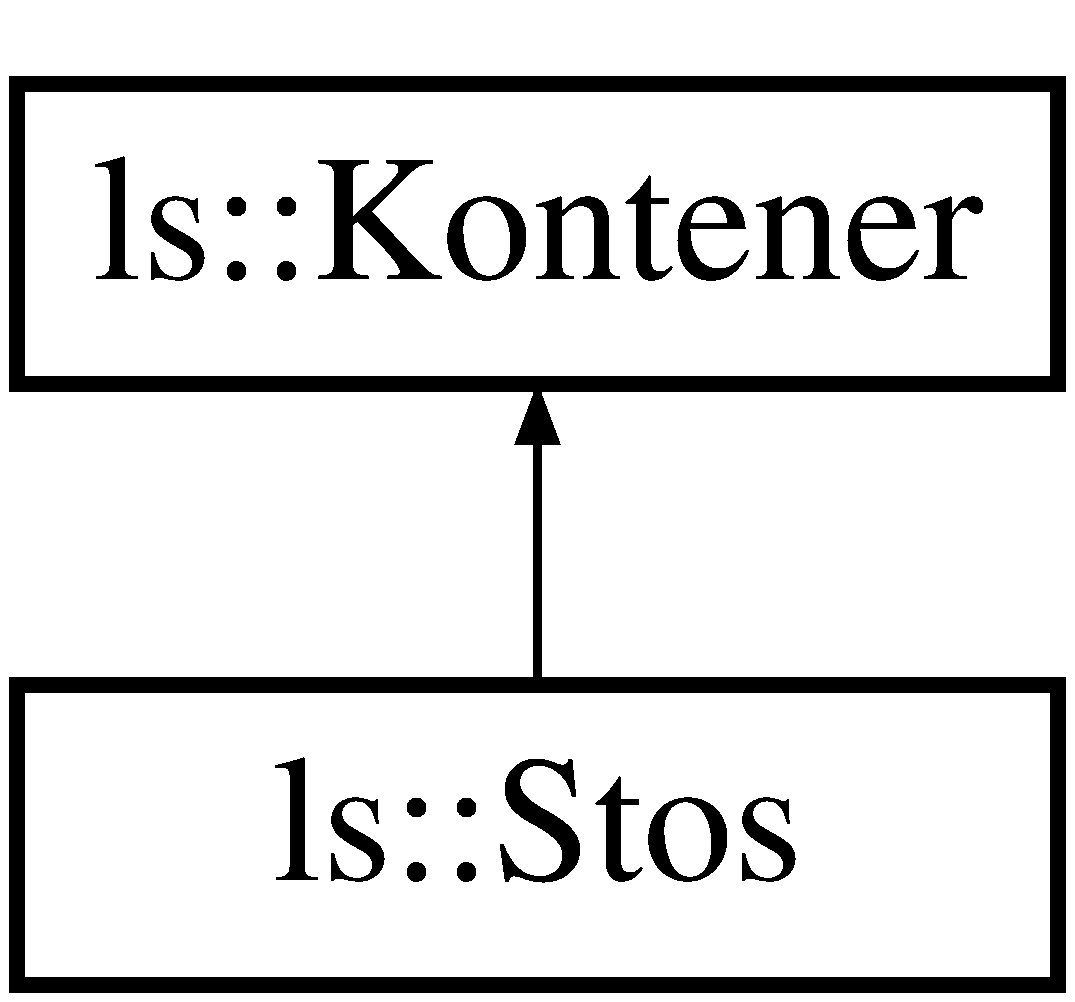
\includegraphics[height=2.000000cm]{classls_1_1_stos}
\end{center}
\end{figure}
\subsection*{Public Member Functions}
\begin{DoxyCompactItemize}
\item 
\hyperlink{classls_1_1_stos_a600e24b908c21f945c451066f84b0bc4}{$\sim$\-Stos} ()
\item 
int \hyperlink{classls_1_1_stos_aba0c11a34e5018a1e96b4822de2c2dfc}{pop} ()
\begin{DoxyCompactList}\small\item\em Pop stosu jaki jest, każdy widzi. Zdejmuje najmłdoszy element i zwraca wartość przez niego przechowywaną. \end{DoxyCompactList}\end{DoxyCompactItemize}
\subsection*{Additional Inherited Members}


\subsection{Detailed Description}


Definition at line 14 of file stos.\-h.



\subsection{Constructor \& Destructor Documentation}
\hypertarget{classls_1_1_stos_a600e24b908c21f945c451066f84b0bc4}{\index{ls\-::\-Stos@{ls\-::\-Stos}!$\sim$\-Stos@{$\sim$\-Stos}}
\index{$\sim$\-Stos@{$\sim$\-Stos}!ls::Stos@{ls\-::\-Stos}}
\subsubsection[{$\sim$\-Stos}]{\setlength{\rightskip}{0pt plus 5cm}ls\-::\-Stos\-::$\sim$\-Stos (
\begin{DoxyParamCaption}
{}
\end{DoxyParamCaption}
)\hspace{0.3cm}{\ttfamily [inline]}}}\label{classls_1_1_stos_a600e24b908c21f945c451066f84b0bc4}


Definition at line 17 of file stos.\-h.



\subsection{Member Function Documentation}
\hypertarget{classls_1_1_stos_aba0c11a34e5018a1e96b4822de2c2dfc}{\index{ls\-::\-Stos@{ls\-::\-Stos}!pop@{pop}}
\index{pop@{pop}!ls::Stos@{ls\-::\-Stos}}
\subsubsection[{pop}]{\setlength{\rightskip}{0pt plus 5cm}int ls\-::\-Stos\-::pop (
\begin{DoxyParamCaption}
{}
\end{DoxyParamCaption}
)\hspace{0.3cm}{\ttfamily [inline]}}}\label{classls_1_1_stos_aba0c11a34e5018a1e96b4822de2c2dfc}


Definition at line 25 of file stos.\-h.



The documentation for this class was generated from the following file\-:\begin{DoxyCompactItemize}
\item 
\hyperlink{stos_8h}{stos.\-h}\end{DoxyCompactItemize}

\hypertarget{classarr_1_1_stos}{\section{arr\-:\-:Stos Class Reference}
\label{classarr_1_1_stos}\index{arr\-::\-Stos@{arr\-::\-Stos}}
}


{\ttfamily \#include $<$stos\-\_\-arr.\-h$>$}

\subsection*{Public Member Functions}
\begin{DoxyCompactItemize}
\item 
\hyperlink{classarr_1_1_stos_acc173736bd233091fe1205c7b2ad08e3}{Stos} ()
\begin{DoxyCompactList}\small\item\em Konstruktor domyślny klasy \hyperlink{classarr_1_1_stos}{Stos}. \end{DoxyCompactList}\item 
\hyperlink{classarr_1_1_stos_a3fa4c0909a0a8af714a7a41925c9bfc4}{Stos} (const \hyperlink{classarr_1_1_stos}{Stos} \&lewy)
\begin{DoxyCompactList}\small\item\em Konstruktor kopiujący klasy \hyperlink{classarr_1_1_stos}{Stos}. \end{DoxyCompactList}\item 
\hyperlink{classarr_1_1_stos_aab930de62382058082057237c0651c85}{$\sim$\-Stos} ()
\begin{DoxyCompactList}\small\item\em Destruktor klasy \hyperlink{classarr_1_1_stos}{Stos}. \end{DoxyCompactList}\item 
void \hyperlink{classarr_1_1_stos_a818b45b7e1133cf8666a8996795823a6}{push} (int val)
\begin{DoxyCompactList}\small\item\em Wrzuca element na szczyt stosu. \end{DoxyCompactList}\item 
int \hyperlink{classarr_1_1_stos_a3d8fd4cebbcc8eb5aed6bfe15e1b86d8}{pop} ()
\begin{DoxyCompactList}\small\item\em Zdejmuje najmłodszy element ze stosu. \end{DoxyCompactList}\item 
bool \hyperlink{classarr_1_1_stos_aa65aee46af4fbfe791b7419d9e2dc2d1}{empty} ()
\begin{DoxyCompactList}\small\item\em Sprawdza, czy stos jest pusty. \end{DoxyCompactList}\item 
int \hyperlink{classarr_1_1_stos_a7f40cb3055b25794dfd484e6e8bd4822}{size} ()
\begin{DoxyCompactList}\small\item\em Zwraca rozmiar stosu. \end{DoxyCompactList}\end{DoxyCompactItemize}
\subsection*{Private Member Functions}
\begin{DoxyCompactItemize}
\item 
void \hyperlink{classarr_1_1_stos_a26833a56e91aefa4dfbc78cafe7ef216}{rozszerz\-\_\-x2} ()
\begin{DoxyCompactList}\small\item\em Metoda zwiększa dwukrotnie pojemnosć stosu. \end{DoxyCompactList}\item 
void \hyperlink{classarr_1_1_stos_a302eb8f0ef06039bd7408a881d3d2c60}{rozszerz\-\_\-1} ()
\begin{DoxyCompactList}\small\item\em Metoda zwiększa pojemnosć stosu o 1. \end{DoxyCompactList}\end{DoxyCompactItemize}
\subsection*{Private Attributes}
\begin{DoxyCompactItemize}
\item 
int $\ast$ \hyperlink{classarr_1_1_stos_ad8e05da5f97f966b3c4f21d661e88b05}{tablica}
\item 
int \hyperlink{classarr_1_1_stos_a1980b721d3a83d8811b07ccf37f62e5e}{rozmiar\-\_\-stosu}
\item 
int \hyperlink{classarr_1_1_stos_a577c49248d0925cb5ca4f0a53aeebe8c}{pojemnosc\-\_\-stosu}
\end{DoxyCompactItemize}


\subsection{Detailed Description}


Definition at line 7 of file stos\-\_\-arr.\-h.



\subsection{Constructor \& Destructor Documentation}
\hypertarget{classarr_1_1_stos_acc173736bd233091fe1205c7b2ad08e3}{\index{arr\-::\-Stos@{arr\-::\-Stos}!Stos@{Stos}}
\index{Stos@{Stos}!arr::Stos@{arr\-::\-Stos}}
\subsubsection[{Stos}]{\setlength{\rightskip}{0pt plus 5cm}arr\-::\-Stos\-::\-Stos (
\begin{DoxyParamCaption}
{}
\end{DoxyParamCaption}
)\hspace{0.3cm}{\ttfamily [inline]}}}\label{classarr_1_1_stos_acc173736bd233091fe1205c7b2ad08e3}


Definition at line 26 of file stos\-\_\-arr.\-h.

\hypertarget{classarr_1_1_stos_a3fa4c0909a0a8af714a7a41925c9bfc4}{\index{arr\-::\-Stos@{arr\-::\-Stos}!Stos@{Stos}}
\index{Stos@{Stos}!arr::Stos@{arr\-::\-Stos}}
\subsubsection[{Stos}]{\setlength{\rightskip}{0pt plus 5cm}arr\-::\-Stos\-::\-Stos (
\begin{DoxyParamCaption}
\item[{const {\bf Stos} \&}]{lewy}
\end{DoxyParamCaption}
)}}\label{classarr_1_1_stos_a3fa4c0909a0a8af714a7a41925c9bfc4}
Bezużyteczny dla trzeciego zadania, ale na pewno kolega się ucieszy. 

Definition at line 3 of file stos\-\_\-arr.\-cpp.

\hypertarget{classarr_1_1_stos_aab930de62382058082057237c0651c85}{\index{arr\-::\-Stos@{arr\-::\-Stos}!$\sim$\-Stos@{$\sim$\-Stos}}
\index{$\sim$\-Stos@{$\sim$\-Stos}!arr::Stos@{arr\-::\-Stos}}
\subsubsection[{$\sim$\-Stos}]{\setlength{\rightskip}{0pt plus 5cm}arr\-::\-Stos\-::$\sim$\-Stos (
\begin{DoxyParamCaption}
{}
\end{DoxyParamCaption}
)}}\label{classarr_1_1_stos_aab930de62382058082057237c0651c85}


Definition at line 10 of file stos\-\_\-arr.\-cpp.



\subsection{Member Function Documentation}
\hypertarget{classarr_1_1_stos_aa65aee46af4fbfe791b7419d9e2dc2d1}{\index{arr\-::\-Stos@{arr\-::\-Stos}!empty@{empty}}
\index{empty@{empty}!arr::Stos@{arr\-::\-Stos}}
\subsubsection[{empty}]{\setlength{\rightskip}{0pt plus 5cm}bool arr\-::\-Stos\-::empty (
\begin{DoxyParamCaption}
{}
\end{DoxyParamCaption}
)}}\label{classarr_1_1_stos_aa65aee46af4fbfe791b7419d9e2dc2d1}
\begin{DoxyReturn}{Returns}
Zwraca prawdę, jeżeli kolejka jest pusta. W przeciwnym razie zwraca false. 
\end{DoxyReturn}


Definition at line 38 of file stos\-\_\-arr.\-cpp.

\hypertarget{classarr_1_1_stos_a3d8fd4cebbcc8eb5aed6bfe15e1b86d8}{\index{arr\-::\-Stos@{arr\-::\-Stos}!pop@{pop}}
\index{pop@{pop}!arr::Stos@{arr\-::\-Stos}}
\subsubsection[{pop}]{\setlength{\rightskip}{0pt plus 5cm}int arr\-::\-Stos\-::pop (
\begin{DoxyParamCaption}
{}
\end{DoxyParamCaption}
)}}\label{classarr_1_1_stos_a3d8fd4cebbcc8eb5aed6bfe15e1b86d8}


Definition at line 32 of file stos\-\_\-arr.\-cpp.

\hypertarget{classarr_1_1_stos_a818b45b7e1133cf8666a8996795823a6}{\index{arr\-::\-Stos@{arr\-::\-Stos}!push@{push}}
\index{push@{push}!arr::Stos@{arr\-::\-Stos}}
\subsubsection[{push}]{\setlength{\rightskip}{0pt plus 5cm}void arr\-::\-Stos\-::push (
\begin{DoxyParamCaption}
\item[{int}]{val}
\end{DoxyParamCaption}
)}}\label{classarr_1_1_stos_a818b45b7e1133cf8666a8996795823a6}


Definition at line 15 of file stos\-\_\-arr.\-cpp.

\hypertarget{classarr_1_1_stos_a302eb8f0ef06039bd7408a881d3d2c60}{\index{arr\-::\-Stos@{arr\-::\-Stos}!rozszerz\-\_\-1@{rozszerz\-\_\-1}}
\index{rozszerz\-\_\-1@{rozszerz\-\_\-1}!arr::Stos@{arr\-::\-Stos}}
\subsubsection[{rozszerz\-\_\-1}]{\setlength{\rightskip}{0pt plus 5cm}void arr\-::\-Stos\-::rozszerz\-\_\-1 (
\begin{DoxyParamCaption}
{}
\end{DoxyParamCaption}
)\hspace{0.3cm}{\ttfamily [private]}}}\label{classarr_1_1_stos_a302eb8f0ef06039bd7408a881d3d2c60}


Definition at line 58 of file stos\-\_\-arr.\-cpp.

\hypertarget{classarr_1_1_stos_a26833a56e91aefa4dfbc78cafe7ef216}{\index{arr\-::\-Stos@{arr\-::\-Stos}!rozszerz\-\_\-x2@{rozszerz\-\_\-x2}}
\index{rozszerz\-\_\-x2@{rozszerz\-\_\-x2}!arr::Stos@{arr\-::\-Stos}}
\subsubsection[{rozszerz\-\_\-x2}]{\setlength{\rightskip}{0pt plus 5cm}void arr\-::\-Stos\-::rozszerz\-\_\-x2 (
\begin{DoxyParamCaption}
{}
\end{DoxyParamCaption}
)\hspace{0.3cm}{\ttfamily [private]}}}\label{classarr_1_1_stos_a26833a56e91aefa4dfbc78cafe7ef216}


Definition at line 43 of file stos\-\_\-arr.\-cpp.

\hypertarget{classarr_1_1_stos_a7f40cb3055b25794dfd484e6e8bd4822}{\index{arr\-::\-Stos@{arr\-::\-Stos}!size@{size}}
\index{size@{size}!arr::Stos@{arr\-::\-Stos}}
\subsubsection[{size}]{\setlength{\rightskip}{0pt plus 5cm}int arr\-::\-Stos\-::size (
\begin{DoxyParamCaption}
{}
\end{DoxyParamCaption}
)\hspace{0.3cm}{\ttfamily [inline]}}}\label{classarr_1_1_stos_a7f40cb3055b25794dfd484e6e8bd4822}


Definition at line 54 of file stos\-\_\-arr.\-h.



\subsection{Member Data Documentation}
\hypertarget{classarr_1_1_stos_a577c49248d0925cb5ca4f0a53aeebe8c}{\index{arr\-::\-Stos@{arr\-::\-Stos}!pojemnosc\-\_\-stosu@{pojemnosc\-\_\-stosu}}
\index{pojemnosc\-\_\-stosu@{pojemnosc\-\_\-stosu}!arr::Stos@{arr\-::\-Stos}}
\subsubsection[{pojemnosc\-\_\-stosu}]{\setlength{\rightskip}{0pt plus 5cm}int arr\-::\-Stos\-::pojemnosc\-\_\-stosu\hspace{0.3cm}{\ttfamily [private]}}}\label{classarr_1_1_stos_a577c49248d0925cb5ca4f0a53aeebe8c}


Definition at line 12 of file stos\-\_\-arr.\-h.

\hypertarget{classarr_1_1_stos_a1980b721d3a83d8811b07ccf37f62e5e}{\index{arr\-::\-Stos@{arr\-::\-Stos}!rozmiar\-\_\-stosu@{rozmiar\-\_\-stosu}}
\index{rozmiar\-\_\-stosu@{rozmiar\-\_\-stosu}!arr::Stos@{arr\-::\-Stos}}
\subsubsection[{rozmiar\-\_\-stosu}]{\setlength{\rightskip}{0pt plus 5cm}int arr\-::\-Stos\-::rozmiar\-\_\-stosu\hspace{0.3cm}{\ttfamily [private]}}}\label{classarr_1_1_stos_a1980b721d3a83d8811b07ccf37f62e5e}


Definition at line 11 of file stos\-\_\-arr.\-h.

\hypertarget{classarr_1_1_stos_ad8e05da5f97f966b3c4f21d661e88b05}{\index{arr\-::\-Stos@{arr\-::\-Stos}!tablica@{tablica}}
\index{tablica@{tablica}!arr::Stos@{arr\-::\-Stos}}
\subsubsection[{tablica}]{\setlength{\rightskip}{0pt plus 5cm}int$\ast$ arr\-::\-Stos\-::tablica\hspace{0.3cm}{\ttfamily [private]}}}\label{classarr_1_1_stos_ad8e05da5f97f966b3c4f21d661e88b05}


Definition at line 10 of file stos\-\_\-arr.\-h.



The documentation for this class was generated from the following files\-:\begin{DoxyCompactItemize}
\item 
\hyperlink{stos__arr_8h}{stos\-\_\-arr.\-h}\item 
\hyperlink{stos__arr_8cpp}{stos\-\_\-arr.\-cpp}\end{DoxyCompactItemize}

\chapter{File Documentation}
\hypertarget{benchmark_8cpp}{\section{benchmark.\-cpp File Reference}
\label{benchmark_8cpp}\index{benchmark.\-cpp@{benchmark.\-cpp}}
}
{\ttfamily \#include \char`\"{}../inc/benchmark.\-h\char`\"{}}\\*
\subsection*{Functions}
\begin{DoxyCompactItemize}
\item 
void \hyperlink{benchmark_8cpp_aa64f5c659f0dd5f25435b15c1e1fa7f5}{Benchmark} ()
\begin{DoxyCompactList}\small\item\em Główna funkcja programu. \end{DoxyCompactList}\item 
int \hyperlink{benchmark_8cpp_a43bc241c88791024a92dc76ff18d0d48}{licz\-\_\-dekady} (int dlugosc\-\_\-ciagu)
\begin{DoxyCompactList}\small\item\em Funkcja pomocnicza do określania ilości dekad. \end{DoxyCompactList}\end{DoxyCompactItemize}


\subsection{Function Documentation}
\hypertarget{benchmark_8cpp_aa64f5c659f0dd5f25435b15c1e1fa7f5}{\index{benchmark.\-cpp@{benchmark.\-cpp}!Benchmark@{Benchmark}}
\index{Benchmark@{Benchmark}!benchmark.cpp@{benchmark.\-cpp}}
\subsubsection[{Benchmark}]{\setlength{\rightskip}{0pt plus 5cm}void Benchmark (
\begin{DoxyParamCaption}
{}
\end{DoxyParamCaption}
)}}\label{benchmark_8cpp_aa64f5c659f0dd5f25435b15c1e1fa7f5}
Funkcja wywoływana w funkcji \hyperlink{main_8cpp_ae66f6b31b5ad750f1fe042a706a4e3d4}{main()}. Nie przyjmuje argumentów ani nie zwraca wartości. Funkcja otwiera plik, który powinien zawierać ciąg danych, na których przeprowadzona zostanie operacja. Otwiera także plik, do którego zapisane mają zostać wyniki czasowe operacji. Nazwy plików określone są w nagłówku \char`\"{}ustawienia.\-h\char`\"{}. Z pliku wejściowego wczytuje do obiektu klasy std\-::vector ciąg danych. Do zmiennej typu clock\-\_\-t zostaje zapisany czas procesora od rozpoczęcia procesu. Do funkcji \hyperlink{operacja_8h_a7de44f86b01513b6593ff27e0f62645e}{operacja()} zostaje przekazana referencja do obiektu zawierającego ciąg danych. Po wyjściu z funkcji \hyperlink{operacja_8h_a7de44f86b01513b6593ff27e0f62645e}{operacja()} do zmiennej typu clock\-\_\-t() zostaje tym razem zapisana różnica czasów procesora pomiędzy rozpoczęciem procesu a wartością typu clock\-\_\-t zwróconą przez funkcję \hyperlink{operacja_8h_a7de44f86b01513b6593ff27e0f62645e}{operacja()}. Czas ten przeliczany jest na sekundy i zapisany do pliku wyjściowego. W \char`\"{}ustawienia.\-h\char`\"{} określona jest ilość powtórzeń pomiaru. Pomiary zaczynają się od operacji na jednej wartości i kończą na ciąu danych o długości największej potęgi dziesiątki. Pomiary powtarzane są co dekadę. Informację o największej potędze dziesiątki dostarcza funkcja \hyperlink{benchmark_8h_a43bc241c88791024a92dc76ff18d0d48}{licz\-\_\-dekady()}. 

Definition at line 4 of file benchmark.\-cpp.

\hypertarget{benchmark_8cpp_a43bc241c88791024a92dc76ff18d0d48}{\index{benchmark.\-cpp@{benchmark.\-cpp}!licz\-\_\-dekady@{licz\-\_\-dekady}}
\index{licz\-\_\-dekady@{licz\-\_\-dekady}!benchmark.cpp@{benchmark.\-cpp}}
\subsubsection[{licz\-\_\-dekady}]{\setlength{\rightskip}{0pt plus 5cm}int licz\-\_\-dekady (
\begin{DoxyParamCaption}
\item[{int}]{dlugosc\-\_\-ciagu}
\end{DoxyParamCaption}
)}}\label{benchmark_8cpp_a43bc241c88791024a92dc76ff18d0d48}
Przyjmuje jako argument liczbę całkowitą reprezentującą długość ciągu danych i zaokrągla ją w dół do najbliższej potęgi liczby 10.


\begin{DoxyParams}[1]{Parameters}
\mbox{\tt in}  & {\em dlugosc\-\_\-ciagu} & Długość ciągu danych. \\
\hline
\end{DoxyParams}
\begin{DoxyReturn}{Returns}
Zwraca zaokrąglenie w dół do najbliższej potęgi dziesiątki wartości dlugosc\-\_\-ciagu. 
\end{DoxyReturn}


Definition at line 59 of file benchmark.\-cpp.


\hypertarget{benchmark_8h}{\section{benchmark.\-h File Reference}
\label{benchmark_8h}\index{benchmark.\-h@{benchmark.\-h}}
}


Deklaracje funkcji związanych z analizą prędkości operacji.  


{\ttfamily \#include \char`\"{}operacja.\-h\char`\"{}}\\*
{\ttfamily \#include \char`\"{}ustawienia.\-h\char`\"{}}\\*
{\ttfamily \#include \char`\"{}kontener.\-h\char`\"{}}\\*
{\ttfamily \#include \char`\"{}stos.\-h\char`\"{}}\\*
{\ttfamily \#include \char`\"{}kolejka.\-h\char`\"{}}\\*
{\ttfamily \#include \char`\"{}stos\-\_\-arr.\-h\char`\"{}}\\*
{\ttfamily \#include $<$fstream$>$}\\*
{\ttfamily \#include $<$iostream$>$}\\*
{\ttfamily \#include $<$vector$>$}\\*
{\ttfamily \#include $<$cstdlib$>$}\\*
{\ttfamily \#include $<$cmath$>$}\\*
\subsection*{Functions}
\begin{DoxyCompactItemize}
\item 
void \hyperlink{benchmark_8h_aa64f5c659f0dd5f25435b15c1e1fa7f5}{Benchmark} ()
\begin{DoxyCompactList}\small\item\em Główna funkcja programu. \end{DoxyCompactList}\item 
int \hyperlink{benchmark_8h_a43bc241c88791024a92dc76ff18d0d48}{licz\-\_\-dekady} (int dlugosc\-\_\-ciagu)
\begin{DoxyCompactList}\small\item\em Funkcja pomocnicza do określania ilości dekad. \end{DoxyCompactList}\end{DoxyCompactItemize}


\subsection{Detailed Description}
Plik zawiera deklaracje funkcji \hyperlink{benchmark_8h_aa64f5c659f0dd5f25435b15c1e1fa7f5}{Benchmark()} oraz \hyperlink{benchmark_8h_a43bc241c88791024a92dc76ff18d0d48}{licz\-\_\-dekady()}. Funkcja \hyperlink{benchmark_8h_aa64f5c659f0dd5f25435b15c1e1fa7f5}{Benchmark()} jest główną funkcją programu benchmarkującego, natomiast funkcja \hyperlink{benchmark_8h_a43bc241c88791024a92dc76ff18d0d48}{licz\-\_\-dekady()} jest funkcją pomocniczą wywoływaną w funkcji \hyperlink{benchmark_8h_aa64f5c659f0dd5f25435b15c1e1fa7f5}{Benchmark()}. 

Definition in file \hyperlink{benchmark_8h_source}{benchmark.\-h}.



\subsection{Function Documentation}
\hypertarget{benchmark_8h_aa64f5c659f0dd5f25435b15c1e1fa7f5}{\index{benchmark.\-h@{benchmark.\-h}!Benchmark@{Benchmark}}
\index{Benchmark@{Benchmark}!benchmark.h@{benchmark.\-h}}
\subsubsection[{Benchmark}]{\setlength{\rightskip}{0pt plus 5cm}void Benchmark (
\begin{DoxyParamCaption}
{}
\end{DoxyParamCaption}
)}}\label{benchmark_8h_aa64f5c659f0dd5f25435b15c1e1fa7f5}
Funkcja wywoływana w funkcji \hyperlink{main_8cpp_ae66f6b31b5ad750f1fe042a706a4e3d4}{main()}. Nie przyjmuje argumentów ani nie zwraca wartości. Funkcja otwiera plik, który powinien zawierać ciąg danych, na których przeprowadzona zostanie operacja. Otwiera także plik, do którego zapisane mają zostać wyniki czasowe operacji. Nazwy plików określone są w nagłówku \char`\"{}ustawienia.\-h\char`\"{}. Z pliku wejściowego wczytuje do obiektu klasy std\-::vector ciąg danych. Do zmiennej typu clock\-\_\-t zostaje zapisany czas procesora od rozpoczęcia procesu. Do funkcji \hyperlink{operacja_8h_a7de44f86b01513b6593ff27e0f62645e}{operacja()} zostaje przekazana referencja do obiektu zawierającego ciąg danych. Po wyjściu z funkcji \hyperlink{operacja_8h_a7de44f86b01513b6593ff27e0f62645e}{operacja()} do zmiennej typu clock\-\_\-t() zostaje tym razem zapisana różnica czasów procesora pomiędzy rozpoczęciem procesu a wartością typu clock\-\_\-t zwróconą przez funkcję \hyperlink{operacja_8h_a7de44f86b01513b6593ff27e0f62645e}{operacja()}. Czas ten przeliczany jest na sekundy i zapisany do pliku wyjściowego. W \char`\"{}ustawienia.\-h\char`\"{} określona jest ilość powtórzeń pomiaru. Pomiary zaczynają się od operacji na jednej wartości i kończą na ciąu danych o długości największej potęgi dziesiątki. Pomiary powtarzane są co dekadę. Informację o największej potędze dziesiątki dostarcza funkcja \hyperlink{benchmark_8h_a43bc241c88791024a92dc76ff18d0d48}{licz\-\_\-dekady()}. 

Definition at line 4 of file benchmark.\-cpp.

\hypertarget{benchmark_8h_a43bc241c88791024a92dc76ff18d0d48}{\index{benchmark.\-h@{benchmark.\-h}!licz\-\_\-dekady@{licz\-\_\-dekady}}
\index{licz\-\_\-dekady@{licz\-\_\-dekady}!benchmark.h@{benchmark.\-h}}
\subsubsection[{licz\-\_\-dekady}]{\setlength{\rightskip}{0pt plus 5cm}int licz\-\_\-dekady (
\begin{DoxyParamCaption}
\item[{int}]{dlugosc\-\_\-ciagu}
\end{DoxyParamCaption}
)}}\label{benchmark_8h_a43bc241c88791024a92dc76ff18d0d48}
Przyjmuje jako argument liczbę całkowitą reprezentującą długość ciągu danych i zaokrągla ją w dół do najbliższej potęgi liczby 10.


\begin{DoxyParams}[1]{Parameters}
\mbox{\tt in}  & {\em dlugosc\-\_\-ciagu} & Długość ciągu danych. \\
\hline
\end{DoxyParams}
\begin{DoxyReturn}{Returns}
Zwraca zaokrąglenie w dół do najbliższej potęgi dziesiątki wartości dlugosc\-\_\-ciagu. 
\end{DoxyReturn}


Definition at line 59 of file benchmark.\-cpp.


\section{/home/damian/mkrawczuk/209147/lab03\-\_\-opt/prj/inc/cegla.h File Reference}
\label{cegla_8h}\index{/home/damian/mkrawczuk/209147/lab03\-\_\-opt/prj/inc/cegla.\-h@{/home/damian/mkrawczuk/209147/lab03\-\_\-opt/prj/inc/cegla.\-h}}


Plik zawiera definicję struktury pomocniczej cegla.  


\subsection*{Classes}
\begin{DoxyCompactItemize}
\item 
struct {\bf cegla}
\begin{DoxyCompactList}\small\item\em Struktura pomocnicza cegla. \end{DoxyCompactList}\end{DoxyCompactItemize}


\subsection{Detailed Description}
Plik zawiera definicję struktury pomocniczej cegla. 

Definition in file {\bf cegla.\-h}.


\section{/home/damian/mkrawczuk/209147/lab03\-\_\-opt/prj/inc/kolejka.h File Reference}
\label{kolejka_8h}\index{/home/damian/mkrawczuk/209147/lab03\-\_\-opt/prj/inc/kolejka.\-h@{/home/damian/mkrawczuk/209147/lab03\-\_\-opt/prj/inc/kolejka.\-h}}


Plik zawiera definicję klasy Kolejka jako pochodnej klasy Kontener oraz definicje jego metod.  


{\ttfamily \#include \char`\"{}kontener.\-h\char`\"{}}\\*
\subsection*{Classes}
\begin{DoxyCompactItemize}
\item 
class {\bf ls\-::\-Kolejka}
\end{DoxyCompactItemize}
\subsection*{Namespaces}
\begin{DoxyCompactItemize}
\item 
{\bf ls}
\begin{DoxyCompactList}\small\item\em \doxyref{Kolejka}{p.}{classls_1_1_kolejka}, abstrakcyjna struktura danych z buforem typu L\-I\-F\-O. \end{DoxyCompactList}\end{DoxyCompactItemize}


\subsection{Detailed Description}
Plik zawiera definicję klasy Kolejka jako pochodnej klasy Kontener oraz definicje jego metod. 

Definition in file {\bf kolejka.\-h}.


\hypertarget{kolejka__arr_8cpp}{\section{kolejka\-\_\-arr.\-cpp File Reference}
\label{kolejka__arr_8cpp}\index{kolejka\-\_\-arr.\-cpp@{kolejka\-\_\-arr.\-cpp}}
}
{\ttfamily \#include \char`\"{}../inc/kolejka\-\_\-arr.\-h\char`\"{}}\\*

\section{/home/damian/mkrawczuk/209147/lab03\-\_\-opt/prj/inc/kolejka\-\_\-arr.h File Reference}
\label{kolejka__arr_8h}\index{/home/damian/mkrawczuk/209147/lab03\-\_\-opt/prj/inc/kolejka\-\_\-arr.\-h@{/home/damian/mkrawczuk/209147/lab03\-\_\-opt/prj/inc/kolejka\-\_\-arr.\-h}}
{\ttfamily \#include $<$cstdlib$>$}\\*
\subsection*{Classes}
\begin{DoxyCompactItemize}
\item 
class {\bf arr\-::\-Kolejka}
\end{DoxyCompactItemize}
\subsection*{Namespaces}
\begin{DoxyCompactItemize}
\item 
{\bf arr}
\end{DoxyCompactItemize}

\hypertarget{kontener_8cpp}{\section{kontener.\-cpp File Reference}
\label{kontener_8cpp}\index{kontener.\-cpp@{kontener.\-cpp}}
}


Plik zawiera definicje metod klasy Kontener.  


{\ttfamily \#include \char`\"{}../inc/kontener.\-h\char`\"{}}\\*

\hypertarget{kontener_8h}{\section{Dokumentacja pliku kontener.\-h}
\label{kontener_8h}\index{kontener.\-h@{kontener.\-h}}
}


Plik zawiera definicję klasy Kontener oraz deklaracje metod tej klasy.  


{\ttfamily \#include $<$cstdlib$>$}\\*
{\ttfamily \#include $<$iostream$>$}\\*
{\ttfamily \#include \char`\"{}cegla.\-h\char`\"{}}\\*
\subsection*{Komponenty}
\begin{DoxyCompactItemize}
\item 
class \hyperlink{classls_1_1_kontener}{ls\-::\-Kontener}
\end{DoxyCompactItemize}
\subsection*{Przestrzenie nazw}
\begin{DoxyCompactItemize}
\item 
\hyperlink{namespacels}{ls}
\begin{DoxyCompactList}\small\item\em \hyperlink{classls_1_1_kolejka}{Kolejka}, abstrakcyjna struktura danych z buforem typu L\-I\-F\-O. \end{DoxyCompactList}\end{DoxyCompactItemize}

\hypertarget{lista__arr_8cpp}{\section{Dokumentacja pliku lista\-\_\-arr.\-cpp}
\label{lista__arr_8cpp}\index{lista\-\_\-arr.\-cpp@{lista\-\_\-arr.\-cpp}}
}
{\ttfamily \#include \char`\"{}../inc/lista\-\_\-arr.\-h\char`\"{}}\\*

\section{/home/damian/mkrawczuk/209147/lab03\-\_\-opt/prj/inc/lista\-\_\-arr.h File Reference}
\label{lista__arr_8h}\index{/home/damian/mkrawczuk/209147/lab03\-\_\-opt/prj/inc/lista\-\_\-arr.\-h@{/home/damian/mkrawczuk/209147/lab03\-\_\-opt/prj/inc/lista\-\_\-arr.\-h}}
{\ttfamily \#include $<$iostream$>$}\\*
\subsection*{Classes}
\begin{DoxyCompactItemize}
\item 
class {\bf arr\-::\-Lista}
\end{DoxyCompactItemize}
\subsection*{Namespaces}
\begin{DoxyCompactItemize}
\item 
{\bf arr}
\end{DoxyCompactItemize}

\hypertarget{main_8cpp}{\section{/home/damian/prog/praca na zajeciach(nowy sort)/prj/src/main.cpp File Reference}
\label{main_8cpp}\index{/home/damian/prog/praca na zajeciach(nowy sort)/prj/src/main.\-cpp@{/home/damian/prog/praca na zajeciach(nowy sort)/prj/src/main.\-cpp}}
}
{\ttfamily \#include \char`\"{}Lista\-Ar.\-h\char`\"{}}\\*
{\ttfamily \#include $<$ctime$>$}\\*
\subsection*{Functions}
\begin{DoxyCompactItemize}
\item 
int \hyperlink{main_8cpp_ae66f6b31b5ad750f1fe042a706a4e3d4}{main} ()
\end{DoxyCompactItemize}


\subsection{Function Documentation}
\hypertarget{main_8cpp_ae66f6b31b5ad750f1fe042a706a4e3d4}{\index{main.\-cpp@{main.\-cpp}!main@{main}}
\index{main@{main}!main.cpp@{main.\-cpp}}
\subsubsection[{main}]{\setlength{\rightskip}{0pt plus 5cm}int main (
\begin{DoxyParamCaption}
{}
\end{DoxyParamCaption}
)}}\label{main_8cpp_ae66f6b31b5ad750f1fe042a706a4e3d4}


Definition at line 7 of file main.\-cpp.


\section{/home/damian/prog/graf/prj/src/operacja.cpp File Reference}
\label{operacja_8cpp}\index{/home/damian/prog/graf/prj/src/operacja.\-cpp@{/home/damian/prog/graf/prj/src/operacja.\-cpp}}


Plik \doxyref{operacja.\-cpp}{p.}{operacja_8cpp}.  


{\ttfamily \#include \char`\"{}operacja.\-h\char`\"{}}\\*
\subsection*{Functions}
\begin{DoxyCompactItemize}
\item 
void {\bf operacja} ({\bf Graf} A, int poczatek, int opcja)
\begin{DoxyCompactList}\small\item\em Funkcja operacja. \end{DoxyCompactList}\end{DoxyCompactItemize}


\subsection{Detailed Description}
Plik \doxyref{operacja.\-cpp}{p.}{operacja_8cpp}. Zawiera definicje funkcji operacja wykonywanej na liscie. 

Definition in file {\bf operacja.\-cpp}.



\subsection{Function Documentation}
\index{operacja.\-cpp@{operacja.\-cpp}!operacja@{operacja}}
\index{operacja@{operacja}!operacja.cpp@{operacja.\-cpp}}
\subsubsection[{operacja}]{\setlength{\rightskip}{0pt plus 5cm}void operacja (
\begin{DoxyParamCaption}
\item[{{\bf Graf}}]{A, }
\item[{int}]{poczatek, }
\item[{int}]{opcja}
\end{DoxyParamCaption}
)}\label{operacja_8cpp_a36acec75c8ad7a4cc3f25f08e27af5c7}


Funkcja operacja. 

Wykonuje zadana operacje na grafie


\begin{DoxyParams}[1]{Parameters}
\mbox{\tt in}  & {\em A} & -\/ Zadany graf o dowolnej ilosci wierzcholkow i krawedzi \\
\hline
\mbox{\tt in}  & {\em poczatek} & -\/ wierzcholek z ktorego zaczynamy przechodzenie Grafu \\
\hline
\mbox{\tt in}  & {\em opcja} & -\/ =1 gdy D\-F\-S =2 gdy B\-S\-F \\
\hline
\end{DoxyParams}


Definition at line 11 of file operacja.\-cpp.


\hypertarget{operacja_8h}{\section{/home/damian/prog/\-Obserwator/prj/inc/operacja.h File Reference}
\label{operacja_8h}\index{/home/damian/prog/\-Obserwator/prj/inc/operacja.\-h@{/home/damian/prog/\-Obserwator/prj/inc/operacja.\-h}}
}
{\ttfamily \#include \char`\"{}Lista\-Ar.\-h\char`\"{}}\\*
\subsection*{Functions}
\begin{DoxyCompactItemize}
\item 
\hyperlink{class_ltab}{Ltab} \hyperlink{operacja_8h_a55fd4ff5b64240f5b5e352bf951d0eaf}{operacja} (\hyperlink{class_ltab}{Ltab} A, int l, int p)
\end{DoxyCompactItemize}


\subsection{Function Documentation}
\hypertarget{operacja_8h_a55fd4ff5b64240f5b5e352bf951d0eaf}{\index{operacja.\-h@{operacja.\-h}!operacja@{operacja}}
\index{operacja@{operacja}!operacja.h@{operacja.\-h}}
\subsubsection[{operacja}]{\setlength{\rightskip}{0pt plus 5cm}{\bf Ltab} operacja (
\begin{DoxyParamCaption}
\item[{{\bf Ltab}}]{A, }
\item[{int}]{l, }
\item[{int}]{p}
\end{DoxyParamCaption}
)}}\label{operacja_8h_a55fd4ff5b64240f5b5e352bf951d0eaf}


Definition at line 10 of file operacja.\-cpp.


\hypertarget{stos_8h}{\section{stos.\-h File Reference}
\label{stos_8h}\index{stos.\-h@{stos.\-h}}
}


Plik zawiera definicję klasy Stos jako pochodnej klasy Kontener oraz definicje jego metod.  


{\ttfamily \#include \char`\"{}kontener.\-h\char`\"{}}\\*
\subsection*{Classes}
\begin{DoxyCompactItemize}
\item 
class \hyperlink{classls_1_1_stos}{ls\-::\-Stos}
\end{DoxyCompactItemize}
\subsection*{Namespaces}
\begin{DoxyCompactItemize}
\item 
\hyperlink{namespacels}{ls}
\begin{DoxyCompactList}\small\item\em \hyperlink{classls_1_1_kolejka}{Kolejka}, abstrakcyjna struktura danych z buforem typu L\-I\-F\-O. \end{DoxyCompactList}\end{DoxyCompactItemize}

\hypertarget{stos__arr_8cpp}{\section{stos\-\_\-arr.\-cpp File Reference}
\label{stos__arr_8cpp}\index{stos\-\_\-arr.\-cpp@{stos\-\_\-arr.\-cpp}}
}
{\ttfamily \#include \char`\"{}../inc/stos\-\_\-arr.\-h\char`\"{}}\\*

\section{/home/damian/mkrawczuk/209147/lab03\-\_\-opt/prj/inc/stos\-\_\-arr.h File Reference}
\label{stos__arr_8h}\index{/home/damian/mkrawczuk/209147/lab03\-\_\-opt/prj/inc/stos\-\_\-arr.\-h@{/home/damian/mkrawczuk/209147/lab03\-\_\-opt/prj/inc/stos\-\_\-arr.\-h}}
{\ttfamily \#include $<$cstdlib$>$}\\*
\subsection*{Classes}
\begin{DoxyCompactItemize}
\item 
class {\bf arr\-::\-Stos}
\end{DoxyCompactItemize}
\subsection*{Namespaces}
\begin{DoxyCompactItemize}
\item 
{\bf arr}
\end{DoxyCompactItemize}

\section{/home/damian/mkrawczuk/209147/lab03\-\_\-opt/prj/inc/ustawienia.h File Reference}
\label{ustawienia_8h}\index{/home/damian/mkrawczuk/209147/lab03\-\_\-opt/prj/inc/ustawienia.\-h@{/home/damian/mkrawczuk/209147/lab03\-\_\-opt/prj/inc/ustawienia.\-h}}


Plik zawiera stałe preprocesora związane z generowaniem, obróbką i pomiarem właściwości danych.  


\subsection*{Macros}
\begin{DoxyCompactItemize}
\item 
\#define {\bf I\-L\-O\-S\-C}~1e2
\item 
\#define {\bf K\-R\-E\-S\-\_\-\-G\-O\-R\-N\-Y}~100
\item 
\#define {\bf K\-R\-E\-S\-\_\-\-D\-O\-L\-N\-Y}~0
\item 
\#define {\bf N\-A\-Z\-W\-A\-\_\-\-P\-L\-I\-K\-U\-\_\-\-W\-E}~\char`\"{}dane.\-dat\char`\"{}
\item 
\#define {\bf N\-A\-Z\-W\-A\-\_\-\-P\-L\-I\-K\-U\-\_\-\-W\-Y}~\char`\"{}arr\-\_\-lista\-\_\-1.\-dat\char`\"{}
\item 
\#define {\bf I\-L\-O\-S\-C\-\_\-\-P\-O\-W\-T\-O\-R\-Z\-E\-N}~10
\end{DoxyCompactItemize}


\subsection{Detailed Description}
Plik zawiera stałe preprocesora związane z generowaniem, obróbką i pomiarem właściwości danych. Makra zawarte w tym pliku służą do sterowania pracą programu generującego dane oraz programu, który te dane przetwarza. Służy też synchronizacji pomiędzy tymi dwoma programami poprzez ujednolicenie nazwy pliku zawierającego dane. 

Definition in file {\bf ustawienia.\-h}.



\subsection{Macro Definition Documentation}
\index{ustawienia.\-h@{ustawienia.\-h}!I\-L\-O\-S\-C@{I\-L\-O\-S\-C}}
\index{I\-L\-O\-S\-C@{I\-L\-O\-S\-C}!ustawienia.h@{ustawienia.\-h}}
\subsubsection[{I\-L\-O\-S\-C}]{\setlength{\rightskip}{0pt plus 5cm}\#define I\-L\-O\-S\-C~1e2}\label{ustawienia_8h_a400f3b16594461b02b7a73ad07b24c0e}
Określa dłuość ciągu danych stworzonych przez program generuj. 

Definition at line 14 of file ustawienia.\-h.

\index{ustawienia.\-h@{ustawienia.\-h}!I\-L\-O\-S\-C\-\_\-\-P\-O\-W\-T\-O\-R\-Z\-E\-N@{I\-L\-O\-S\-C\-\_\-\-P\-O\-W\-T\-O\-R\-Z\-E\-N}}
\index{I\-L\-O\-S\-C\-\_\-\-P\-O\-W\-T\-O\-R\-Z\-E\-N@{I\-L\-O\-S\-C\-\_\-\-P\-O\-W\-T\-O\-R\-Z\-E\-N}!ustawienia.h@{ustawienia.\-h}}
\subsubsection[{I\-L\-O\-S\-C\-\_\-\-P\-O\-W\-T\-O\-R\-Z\-E\-N}]{\setlength{\rightskip}{0pt plus 5cm}\#define I\-L\-O\-S\-C\-\_\-\-P\-O\-W\-T\-O\-R\-Z\-E\-N~10}\label{ustawienia_8h_a923942350ba378e49a53193355cb5ec0}
Tyle razy zostanie powtórzoy pomiar dla jednego zestawu danych. 

Definition at line 24 of file ustawienia.\-h.

\index{ustawienia.\-h@{ustawienia.\-h}!K\-R\-E\-S\-\_\-\-D\-O\-L\-N\-Y@{K\-R\-E\-S\-\_\-\-D\-O\-L\-N\-Y}}
\index{K\-R\-E\-S\-\_\-\-D\-O\-L\-N\-Y@{K\-R\-E\-S\-\_\-\-D\-O\-L\-N\-Y}!ustawienia.h@{ustawienia.\-h}}
\subsubsection[{K\-R\-E\-S\-\_\-\-D\-O\-L\-N\-Y}]{\setlength{\rightskip}{0pt plus 5cm}\#define K\-R\-E\-S\-\_\-\-D\-O\-L\-N\-Y~0}\label{ustawienia_8h_a6b2bdad24a7530210341c1c3a0197dd9}
Określa najmniejszą możliwą liczbę do wygenerowania. 

Definition at line 18 of file ustawienia.\-h.

\index{ustawienia.\-h@{ustawienia.\-h}!K\-R\-E\-S\-\_\-\-G\-O\-R\-N\-Y@{K\-R\-E\-S\-\_\-\-G\-O\-R\-N\-Y}}
\index{K\-R\-E\-S\-\_\-\-G\-O\-R\-N\-Y@{K\-R\-E\-S\-\_\-\-G\-O\-R\-N\-Y}!ustawienia.h@{ustawienia.\-h}}
\subsubsection[{K\-R\-E\-S\-\_\-\-G\-O\-R\-N\-Y}]{\setlength{\rightskip}{0pt plus 5cm}\#define K\-R\-E\-S\-\_\-\-G\-O\-R\-N\-Y~100}\label{ustawienia_8h_a2e9c0e30a722750fa4380b8150337c6f}
Określa największą możliwą liczbę do wygenerowania. 

Definition at line 16 of file ustawienia.\-h.

\index{ustawienia.\-h@{ustawienia.\-h}!N\-A\-Z\-W\-A\-\_\-\-P\-L\-I\-K\-U\-\_\-\-W\-E@{N\-A\-Z\-W\-A\-\_\-\-P\-L\-I\-K\-U\-\_\-\-W\-E}}
\index{N\-A\-Z\-W\-A\-\_\-\-P\-L\-I\-K\-U\-\_\-\-W\-E@{N\-A\-Z\-W\-A\-\_\-\-P\-L\-I\-K\-U\-\_\-\-W\-E}!ustawienia.h@{ustawienia.\-h}}
\subsubsection[{N\-A\-Z\-W\-A\-\_\-\-P\-L\-I\-K\-U\-\_\-\-W\-E}]{\setlength{\rightskip}{0pt plus 5cm}\#define N\-A\-Z\-W\-A\-\_\-\-P\-L\-I\-K\-U\-\_\-\-W\-E~\char`\"{}dane.\-dat\char`\"{}}\label{ustawienia_8h_a38a14ca65ed113a739420d7a6813c0e8}
Określa jak nazywa się plik wygenerowany przez program 'generuj', jednocześnie pliku o tej nazwie poszukuje program 'program' w katalogu, w którym został uruchomiony. 

Definition at line 20 of file ustawienia.\-h.

\index{ustawienia.\-h@{ustawienia.\-h}!N\-A\-Z\-W\-A\-\_\-\-P\-L\-I\-K\-U\-\_\-\-W\-Y@{N\-A\-Z\-W\-A\-\_\-\-P\-L\-I\-K\-U\-\_\-\-W\-Y}}
\index{N\-A\-Z\-W\-A\-\_\-\-P\-L\-I\-K\-U\-\_\-\-W\-Y@{N\-A\-Z\-W\-A\-\_\-\-P\-L\-I\-K\-U\-\_\-\-W\-Y}!ustawienia.h@{ustawienia.\-h}}
\subsubsection[{N\-A\-Z\-W\-A\-\_\-\-P\-L\-I\-K\-U\-\_\-\-W\-Y}]{\setlength{\rightskip}{0pt plus 5cm}\#define N\-A\-Z\-W\-A\-\_\-\-P\-L\-I\-K\-U\-\_\-\-W\-Y~\char`\"{}arr\-\_\-lista\-\_\-1.\-dat\char`\"{}}\label{ustawienia_8h_af22a754e002d9be8ee0b6d97eb9a9882}
Tak nazywać się będzie wygenerowany przez program 'program' plik z wynikami przeprowadzonych pomiarów. 

Definition at line 22 of file ustawienia.\-h.


%--- End generated contents ---

% Index
\newpage
\phantomsection
\addcontentsline{toc}{chapter}{Index}
\printindex

\end{document}
